%Hauptdokument der Erstsemesterzeitschrift "Erste" der Fachgruppe Informatik
\documentclass[
  %final,
  a4paper,              % DIN A4
  style=screen,
  twoside,
  nexus,                % corporate design font
  bookmarkpackage=false
]{tubsartcl}

\usepackage[utf8]{inputenc}
\usepackage{graphicx}
\usepackage{amssymb}
%\usepackage[T1]{fontenc}
\usepackage{multicol}
\usepackage{comment}
\usepackage[ngerman]{babel}
\usepackage{wrapfig}
\usepackage[babel,german=quotes]{csquotes}
\usepackage[obeyFinal]{todonotes}
\usepackage{etoolbox}
\usepackage{sectsty}
\usepackage[hidelinks]{hyperref}
\usepackage{tabularx}
\usepackage{pdfpages}
\usepackage{varwidth}
\usepackage{enumitem}
\usepackage{eurosym}
\usepackage{footnote}
\usepackage{booktabs}

\usetikzlibrary{patterns}

%\KOMAoptions{twoside, headsepline}
\usepackage{geometry}

\geometry{margin=1.5cm}
\geometry{twoside}
%\geometry{bindingoffset=7mm}
\geometry{includehead} 
\geometry{includefoot}
\geometry{footnotesep=2em}
\geometry{footskip=\footskip-2em}
\geometry{headsep=1em}
\geometry{head=5em}
\geometry{nofoot}

%layout-experimente
\setlength{\columnsep}{20pt}
\pagestyle{useheadings}



% Toggles between winter term and summer term 
\newtoggle{winter}

% This system is meant to make updating the Erste for the new semster simple. Every semster gets a new version number that is larger than the previous one (assigned in config.tex). 
% By using \tocheck, defined below, todos can be left in the source and disabled one by one by incresing the version number of the tocheck. Once all todos are adressed, the new version can be released. Later all todos can be enabled again by incrementing the version number.
\newcounter{version}

% Defines a conditional todo. 2 mandatory arguments:
% 1st param, Valid to version: This todo has been adressd as of the given version
% 2nd param, Todo description: What needs to be done to adress this todo
\newrobustcmd{\tocheck}[2]{
	\ifnumless{#1}{\value{version}}{
		\todo[inline]{#2}
	}{}
}

% Versioned url. 2 mandatory arguments:
% 1st param, Valid to version: This url is still valid as of version
% 2nd param, URL: The url
\newrobustcmd{\verUrl}[2]{\ifnumless{#1}{\value{version}}{\todo[inline]{Check \url{#2}}}{}\url{#2}}
\newrobustcmd{\verHref}[4][]{\ifnumless{#2}{\value{version}}{\todo[inline]{Check \url{#3}}}{}\href[#1]{#3}{\nolinkurl{#4}}}

\newrobustcmd{\fginfoUrl}[0]{\verUrl{7}{https://fginfo.tu-braunschweig.de}}

%%

\newrobustcmd{\xkcd}[2]{
	\begin{center}
		\includegraphics[#1]{bilder/XKCD/#2}
	\end{center}
}


% creates a blank page

\newcommand{\blankpage}{
	\newpage
	\thispagestyle{empty}
	\mbox{}
	\newpage
}


% creates a stundenplan
\newenvironment{stundenplan}[6]{%
	\newcommand{\wTag}{#1/6}%
	\newcommand{\hPlan}{#2}%
	\newcommand{\hAbendHeader}{.5}%
	\newcommand{\hAbend}{1.6}%
	\newcommand{\tStart}{zeit(#3,#4)}%
	\newcommand{\tEnde}{zeit(#5,#6)}%

	\pgfmathdeclarefunction{zeit}{2}{\pgfmathparse{##1 + ##2 / 60}}%
	\pgfmathdeclarefunction{tmpYZeit}{1}{\pgfmathparse{-\hPlan * (##1-\tStart) / (\tEnde-\tStart)}}%
	\pgfmathdeclarefunction{yZeit}{1}{\pgfmathparse{%
		max(min(tmpYZeit(##1), tmpYZeit(\tStart)), tmpYZeit(\tEnde)-\hAbendHeader-\hAbend)%
	}}%

%
	\tikzset{%
	  termin/.style={%
	   anchor=north west,%
	   align=left,%
	   %execute at begin node=\setlength{\baselineskip}{1.2em}%
	  }%
	}%

	\newcommand{\tNode}[2]{%
		\node [termin] at (TERMIN) {%
			\begin{varwidth}{1cm*\wTag - .2cm}%
			##1\\%
			\scriptsize ##2%
			\end{varwidth}%
		};%
	}%

%
	\newcommand{\Termin}[8]{%
		%1: Beschreibung, 2: Ort, 3: Tag, 4: Start Stunde, 5: Start Minute, 6: Ende Stunde, 7: Ende Minute, 8: Farbe %
		\draw [##8](\wTag * ##3,{yZeit(zeit(##4,##5))}) coordinate (TERMIN) rectangle (##3  * \wTag + \wTag,{yZeit(zeit(##6,##7))});%
		\tNode{##1}{##2}%
	}%

	\newcommand{\termin}[8]{%
		%1: Beschreibung, 2: Ort, 3: Tag, 4: Start Stunde, 5: Start Minute, 6: Ende Stunde, 7: Ende Minute, 8: Farbe (Fügt Zeit automatisch in Beschreibung ein)%
		\Termin{##1}{##4:##5 -- ##6:##7\ifstrempty{##2}{}{, ##2}}{##3}{##4}{##5}{##6}{##7}{##8}%
	}%

	\newcommand{\abendtermin}[4]{%
		%1: Beschreibung, 2: Ort, 3: Tag, 4: Farbe%
		\draw [##4](\wTag * ##3,-\hPlan-\hAbendHeader) coordinate (TERMIN) rectangle (##3  * \wTag + \wTag, -\hPlan-\hAbendHeader-\hAbend);%
		\tNode{##1}{##2}%
	}%
	\begin{tikzpicture}[font=\small]%
	% spalten
	\foreach \x in {0,...,5}{
		\draw (\x*\wTag,0) -- (\x*\wTag,-\hPlan);
		\draw (\x*\wTag,-\hPlan-\hAbendHeader) -- (\x*\wTag,-\hPlan-\hAbendHeader-\hAbend);
	}
	\draw (6*\wTag,0) -- (6*\wTag,-\hPlan-\hAbendHeader-\hAbend);

	\draw (0,0)--(6*\wTag,0);
	\draw (0, -\hPlan) coordinate (ABEND) rectangle (5*\wTag, -\hPlan-\hAbendHeader);
	\node [anchor=north west,align=center,minimum width=5cm*\wTag] at (ABEND) {\scriptsize \emph{Abend}};
	\draw (0, -\hPlan-\hAbendHeader-\hAbend)--(6*\wTag, -\hPlan-\hAbendHeader-\hAbend);

	\node [anchor=south] at (.5* \wTag,0) {\textbf{Montag}};
	\node [anchor=south] at (1.5* \wTag,0) {\textbf{Dienstag}};
	\node [anchor=south] at (2.5* \wTag,0) {\textbf{Mittwoch\vphantom{g}}};
	\node [anchor=south] at (3.5* \wTag,0) {\textbf{Donnerstag}};
	\node [anchor=south] at (4.5* \wTag,0) {\textbf{Freitag}};
	\node [anchor=south] at (5.5* \wTag,0) {\textbf{Wochenende\vphantom{g}}};
}{\end{tikzpicture}}

\renewcommand{\familydefault}{\sfdefault}

%\clubpenalty = 10000
%\widowpenalty = 10000 
%\displaywidowpenalty = 10000

% Trennregeln
\hyphenation{
	AStA
	Mit-be-wohnerIn-nen
	Pro-fessorInnen
	erwischt
	viiieel
	y-Nummer
	Uniaccount
	Andreas-berg
}

% left aligned sections
%\allsectionsfont{\raggedright}


\settoggle{winter}{false}
\setcounter{version}{7}



\begin{document}
	\thispagestyle{empty}

	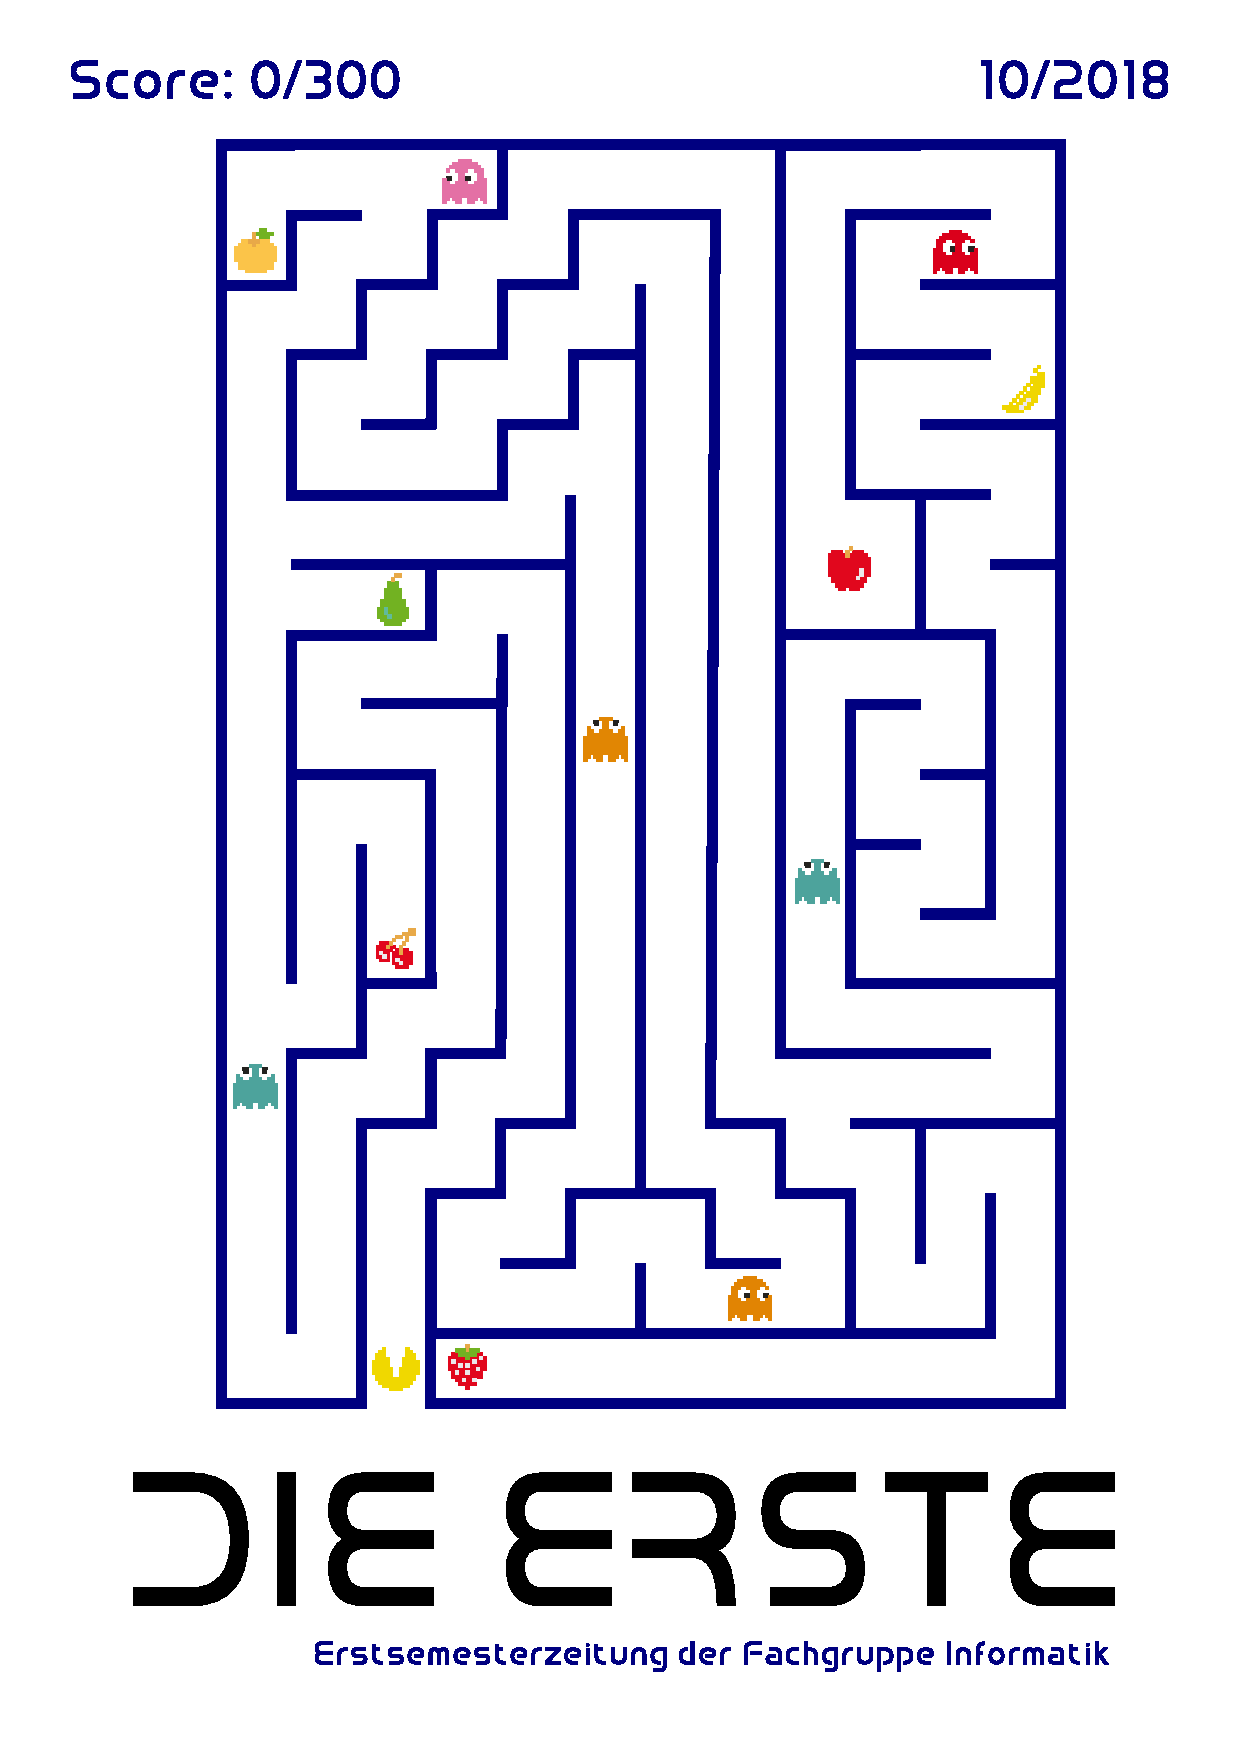
\includepdf[pages={1}]{bilder/Erste_Cover/cover.pdf}

	\newpage
	\tocheck{7}{Update date on cover}
	
	\thispagestyle{empty}
	\listoftodos
	\vspace*{2.5cm}
	\xkcd{width=0.9\textwidth}{tech_support_cheat_sheet}

	\newpage

	\setcounter{page}{1}
	\tableofcontents

	\vfill
	\xkcd{width=\textwidth}{sail}

	\newpage

	\input{texte/vorwort}

	\vfill
	\xkcd{width=.7\textwidth}{dorm_poster}

	\newpage

	\section{Die ersten Tage}
		% !TEX root = ../../1-te.tex

\subsection{Checkliste}
\label{checkliste}
	Hier wird zusammengefasst, was du in den ersten Tagen des Studiums unbedingt erledigen solltest. Wenn du die ToDos auf der Checkliste nach Erledigung abhakst, verlierst du nicht den Überblick und vergisst nichts.
	
%\vspace*{0.5cm}
% !TEX root = ../../1-te.te2

\begin{center}
\begin{tabularx}{\textwidth}{|p{3mm}|X|p{7.4cm}|c|c|}
\hline $\checkmark$ 
       & \textbf{Todo}             & \textbf{Zu erledigen bis}                                  & \textbf{Seite}               & \textbf{Muss?} \\ 
\hline & BAföG beantragen          & Spätestens Ende \iftoggle{winter}{Oktober}{April}          & \pageref{todobafoeg}         & optional \\ 
\hline & Wohnsitz ummelden         & 1 Woche nach Umzug                                         & \pageref{todoummelden}       & ja \\
\hline & Mailinglisten             & So früh wie möglich                                        & \pageref{mailinglisten}      & ja \\ 
\hline & Studiengrobplanung        & Vor dem Stundenplan bauen                                  & \pageref{grob}               & ja \\
\hline & Auflagen klären           & So früh wie möglich, final: Ende 2. Semester               & \pageref{auflagen}           & Master \\ 
\hline & Persönlicher Stundenplan  & 04.04.2018, 10:00 Uhr mit der Fachgruppe                   & \pageref{masterstundenplan}  & ja \\ 
\hline & TAN-Liste organisieren    & Möglichst vor Prüfungsanmeldezeitraum                      & \pageref{todoanmeldung}      & ja \\ 
\hline & Prüfungsanmeldung         & im Prüfungsanmeldezeitraum                                 & \pageref{todoanmeldung}      & ja \\ 
\hline & Blog abonnieren           & So früh wie möglich                                        & \pageref{fachgruppe}         & ja \\ 
\hline & Prüfungsordnung lesen     & Zu den ersten Klausuren                                    & \pageref{po}                 & ja \\ 
\hline & TUcard validieren         & Zu Beginn und zu jedem neuen Semester                      & \pageref{tucard}             & ja \\
\hline & Bibliotheksausweis        & Vor der ersten Buchausleihe                                & \pageref{todobib}            & optional \\
\hline & Stud.IP-Nachrichten weiterleiten  & Wenn man nichts verpassen möchte                   & \pageref{studipfwd}          & optional \\
\hline
\end{tabularx} 
\end{center}
\tocheck{7}{Exakte Daten Anmeldewoche einfügen, s.\url{https://www.tu-braunschweig.de/fk1/service/informatik/pa}}


\begin{multicols}{2}
\raggedcolumns

\subsubsection{BAföG}
	\label{todobafoeg}
	Wer Studierendenförderung nach dem Bundesausbildungsförderungsgesetz (BAföG) beantragen möchte, sollte sich am besten gründlich informieren: \verHref{7}{https://www.xn--bafg-7qa.de}{https://www.bafög.de}
 
	Förderungsanträge gibt es zum Download oder in Papierform im EG des Amtes für Ausbildungsförderung in der Wilhelmstraße 1. Wenn du BAföG beantragen möchtest, stelle den Antrag so früh wie möglich, denn es wird nicht rückwirkend gezahlt.

	Zum Anfang des Semester ist mit längeren Wartezeiten zu rechnen, im Notfall kannst du beim AStA-Sozialreferat ein kurzfristiges, zinsloses Darlehen beantragen, um den ersten Monat zu überbrücken. Das Darlehen ist auf 450 Euro begrenzt und muss spätestens nach drei Monaten zurückgezahlt werden. Mehr Informationen findest du auf der Seite des Sozialreferats: \verUrl{7}{https://www.asta.tu-braunschweig.de/referate/sozialreferat/}


\subsubsection{Ummelden}
	\label{todoummelden}

	Wer neu nach Braunschweig gezogen ist, muss sich innerhalb einer Woche beim Einwohnermeldeamt anmelden. Wenn du die Frist verpasst, drohen theoretisch Strafen, aber praktisch sieht es da nicht so streng aus. Wenn man Braunschweig als Erstwohnsitz wählt, bekommt man (ein Jahr später) eine einmalige Zuzugsprämie von 100 Euro (Immatrikulationsbescheinigung nicht vergessen). Alternativ kann man Braunschweig auch als Zweitwohnsitz wählen.

\subsubsection{Prüfungsanmeldung}
	\label{todoanmeldung}

	Du musst dich für alle Prüfungen, an denen du teilnehmen willst, vorher beim Prüfungsamt anmelden.
Die Fristen sind relativ früh im Semester und werden auf den Seiten des Prüfungsamtes (\verUrl{7}{https://www.tu-braunschweig.de/fk1/service/informatik/pa}) veröffentlicht und über die Mailingliste kommuniziert.
Prüfungen können im Prüfungsanmeldezeitraum schriftlich im Prüfungsamt oder online über das QIS-Portal (\verUrl{7}{https://vorlesungen.tu-braunschweig.de}) angemeldet werden.

	Für die Online-Anmeldung benötigst du eine TAN-Liste, die du dir vorher im Prüfungsamt organisieren musst. Es empfiehlt sich, dies bereits vor dem Prüfungsanmeldezeitraum zu erledigen, da das Prüfungsamt dann meist weniger ausgelastet ist.

	Unter folgendem Link findest du außerdem alle Prüfungstermine für die Informatik:
	\verUrl{7}{https://www.tu-braunschweig.de/fk1/service/informatik/pa}

\subsubsection{TUcard}
	\label{tucard}
	
	Alle Studierenden der TU erhaten den elektronischen Studierendenausweis TUcard, der auch als Bibliotheksausweis, Mensakarte und Semesterticket genutzt werden kann.

	Damit die Karte gültig ist, muss sie zu Beginn und zu jedem neuen Semester validiert werden. Das bedeutet, dass der Thermostreifen auf der Karte in einem Validierungsdrucker mit den aktuellen Daten beschrieben werden muss.

	Das Börsenguthaben der Karte, beispielsweise zum Bezahlen in der Mensa, kann an Börsenaufwertern aufgeladen werden.

	Zum Drucken kann Guthaben der Karte auf ein Druckkonto umgebucht werden. Dies geschieht an den Druckkontenumbuchern.

	Weitere Informationen zur TUcard findest du unter: \verUrl{7}{https://www.tu-braunschweig.de/studium/imstudium/tucard}

\subsubsection{Uni-Bibliothek}
	\label{todobib}

	Um Bücher in der Universitätsbibliothek (UB) ausleihen zu können, muss deine TUcard für die Nutzung als Bibliotheksausweis freigeschaltet werden. Dafür stellst du an einem der Terminals direkt in der Bibliothek oder online einen Antrag, die Freischaltung erfolgt dann am Schalter in der Bibliothek. Je nachdem, ob du zu Beginn schon Bücher brauchst, kannst du die Funktion auch später aktivieren.

	In der Bibliothek stehen außerdem Kopierer bereit, die du nutzen kannst. Einen davon kannst du mit Kleingeld befüllen, kompfortabler geht es aber mit einer Kopierkarte. Die bekommst du für ein paar Euro in der Bibliothek. Zu Semesterbeginn gibt es oft noch Einführungskurse in die Bibliotheksbenutzung.
\end{multicols}

		% !TEX root = ../../1-te.tex

\subsection{Wichtige Termine am Anfang des Studiums}

\tocheck{8}{Termine für aktuelle O-Woche einfügen}

Wir möchten den Start an der TU Braunschweig so gut wie möglich begleiten. Daher wird es zu Beginn des Semesters wieder Begrüßungs- und Einführungsveranstaltungen geben. Eine Übersicht über die Termine findest du auch auf der Rückseite dieser Zeitschrift. Das System der Raumnummern ist auf Seite \pageref{campuskarte} erklärt.

Bis zum Semesterstart können sich einzelne Termine noch ändern. Den ganz aktuellen Stand gibt es online unter \verUrl{8}{https://fginfo.tu-braunschweig.de/ersti/}.

\renewcommand{\labelitemi}{$\bullet$}
\renewcommand{\labelitemii}{$\bullet$}
\renewcommand{\labelitemiii}{$\bullet$}
\renewcommand{\labelitemiv}{$\bullet$}

\begin{itemize}
    \item Montag, 14. Oktober
        \begin{itemize}
            \item 10:00 Uhr: Gemeinsames Frühstück (Plaza, IZ 1.OG) \textbf{Bitte eigenes Geschirr, Becher (für Kaffee o.ä.) und Besteck mitbringen}
            \item 11:00 Uhr: Info-Vortrag \& Stundenplanbau-Workshop (IZ 160)
            \item \textit{13:00 - 17:00 Uhr: Vorkurs}
        \end{itemize}
    \item Dienstag, 15. Oktober
        \begin{itemize}
            \item \textit{9:00 - 13:00 Uhr: Vorkurs}
            \item 13:00 Uhr: Mensabesuch (Mensa 1)
            \item 14:00 Uhr: Campustour (Treffen Fachgruppenraum Informatik, Foyer IZ)
        \end{itemize}
    \item Mittwoch, 16. Oktober
        \begin{itemize}
            \item \textit{9:00 - 13:00 Uhr: Vorkurs}
            \item 14:00 Uhr: Nachmittagsprogramm, du kannst zwischen mehreren Optionen auswählen
            \item 17:00 Uhr: Linux-Install-Party (IZ 161)\footnote{Weitere Infos: \verUrl{8}{https://wiki.fginfo.tu-bs.de/doku.php?id=events:linux}}
        \end{itemize}
    \item Donnerstag,  17. Oktober
        \begin{itemize}
            \item \textit{9:00 - 13:00 Uhr: Vorkurs}
            \item 14:00 Uhr: Nachmittagsprogramm, du kannst zwischen mehreren Optionen auswählen
            \item 19:00 Uhr: Kneipentour (Start Haupteingang der Mensa 1)
        \end{itemize}
    \item Freitag, 18. Oktober
        \begin{itemize}
            \item \textit{11:00 - 16:00 Uhr: Vorkurs}
        \end{itemize}
    \item Montag, 21. Oktober
        \begin{itemize}
            \item \textit{9:00 Uhr: Zentrale Begrüßung aller Erstsemester (Eintracht-Stadium)}
            \item \textit{10:30 – 12:00 Uhr: Infobörse „Studium ist mehr“ (Foyer von Altgebäude und Audimax)}
            \item \textit{11:30 – 13:00 Uhr: Vorlesung: Lineare Algebra (PK 2.2)}
            \item \textit{13:15 - 14:15 Uhr: Erstibegrüßung der Informatik (PK 2.1)}
            \item \textit{22:00 Uhr: Uniweite Erstiparty (Millenium Event-Center, Madamenweg 77)}
        \end{itemize}
    \item Dienstag, 22. Oktober
        \begin{itemize}
            \item \textit{13:15 - 14:45 Uhr: Übung: Diskrete Mathematik (PK 2.2)}
        \end{itemize}
    \item Mittwoch, 23. Oktober
        \begin{itemize}
            \item \textit{9:45 - 11:15 Uhr: Vorlesung: Diskrete Mathematik (PK 11.2)}
            \item \textit{15:00 – 16:30 Uhr: Vorlesung: Lineare Algebra für Informatiker (PK 2.2)}
            \item 19:00 Uhr: Analoger Spieleabend (Flur vor IZ 150)
        \end{itemize}
    \item Donnerstag, 24. Oktober
        \begin{itemize}
            \item \textit{keine Termine}
        \end{itemize}
    \item Freitag, 25. Oktober
        \begin{itemize}
            \item \textit{9:45 – 11:15 Uhr: Übung: Lineare Algebra für Informatiker (PK 2.2)}
            \item \textit{13:00 Uhr: Treffen der Medizininformatiker (IZ 404) \textbf{Nur für Medizininformatikstudierende. Um Anmeldung wird gebeten, wenn du Medizininformatik studierest und teilnehmen willst, schicke eine Mail an ute.zeisberg@plri.de}}
            \item 14:30 Uhr: Treffen Abfahrt Erstifahrt (Foyer IZ, Mühlenpfordstraße 23)
        \end{itemize}
    \item Ersti-Wochenende
        \begin{itemize}
            \item Wann? \textit{25. – 27. Oktober}
            \item Wo? Naturfreundehaus Eichsfelder Hütte (St. Andreasberg)
            \item Was? Lerne deine Mitstudierenden kennen, habe Spaß :)
            \item Finanzierung? Größtenteils aus Studienqualitätsmitteln, dazu ein kleiner Selbstkostenbeitrag
            \item Fristen: \textit{Anmeldung und Bezahlung des Selbstkostenbeitrags bis 23. Oktober}
            \item Du kannst dich unter folgender Adresse für die Erstifahrt anmelden: \verUrl{8}{https://tickets.fginfo.tu-bs.de/fginfo/efws19/}
        \end{itemize}
    \end{itemize}

	\newpage

	\section{Studienplan(ung) für jeden}
		\label{studienplan}
		\begin{multicols}{2}
		\input{texte/studienplan/verantwortung} % Verantwortung
		\input{texte/studienplan/bachmast}  % Bachelor und Master (Herden und Rudel)
		% !TEX root = ../../1-te.tex

\subsection{Die Prüfungsordnung}
\label{po}
	An einer Universität gibt es tausende Regeln und Ordnungen. Die wichtigste ist die Prüfungsordnung: Sie enthält Antworten auf 95\% aller Fragen, die im Studium auftreten - nicht nur, wenn es um die eigentlichen Prüfungen geht. Die genaue Bezeichnung lautet \emph{Besonderer Teil der Prüfungsordnung für den Bachelor-/Masterstudiengang Informatik der Technischen Universität Braunschweig}. Und da sie weder besonders lang, noch kompliziert geschrieben ist, sollten sie alle Studierenden mindestens einmal lesen.

	Dann gibt es noch die APO, die Allgemeine Prüfungsordnung. Sie gilt uniweit für alle Studiengänge, doch die beiden BPOs überschreiben die meisten APO-Regelungen.

	Wenn du es noch nicht getan hast, lade dir deine aktuelle Prüfungsordnung am besten von \verUrl{8}{http://www.tu-braunschweig.de/fk1/service/informatik/dokumente} herunter.


   % Prüfungsordnung
		% !TEX root = ../../1-te.tex

\subsection{Module und Co.}
	Um deinen Abschluss zu bekommen, musst du eine vordefinierte Menge von Modulen abdecken. Ein Modul besteht aus verschiedenen Bestandteilen.

\subsubsection{Vorlesung, Übung, etc.}
	\paragraph*{Vorlesung}
	Vorlesungen werden vor allen Studis abgehalten und befassen sich in erster Linie mit der theoretischen Herleitung des Stoffes. Solltest du in der Vorlesung einmal etwas nicht verstehen, so ist das nicht so tragisch. Vorlesungen an der Uni unterscheiden sich stark vom Unterricht an der Schule. Gehe nicht davon aus, Vorlesungsinhalte direkt zu verstehen. Plane eine gewisse Nachbearbeitungszeit für die Vorlesungen ein. In einer Vorlesung ist wegen der großen Teilnehmerzahl normalerweise kein Dialog mit dem oder der Vortragenden möglich. Aufgetretene Fragen können und sollten am besten direkt nach der Vorlesung oder sonst in einer Sprechstunde mit der oder dem Lehrenden geklärt werden.
	
	\paragraph*{Große Übung}
	Ergänzend gibt es die großen Übungen, auch Saalübungen genannt. Diese finden, wie die Vorlesung, vor dem gesamten Auditorium statt und sollen das erworbene, theoretische Wissen vertiefen und vor allem auch praktische, klausurbezogene Anwendungen aufzeigen. Die große Übung wird normalerweise von einer Mitarbeiterin oder einem Mitarbeiter gehalten. Sie sind bei  fachlichen Fragen kompetente Ansprechpartner/innen und meistens auch sehr hilfsbereit. Da sie  üblicherweise die Klausuren entwerfen, kann man bei genauem Hinhören in den großen Übungen oder im privaten Gespräch mit ihnen einiges über die Prüfung erfahren.

	\paragraph*{Kleine Übung, Seminargruppe}
	Als erstes eine Warnung: Kleine Übungen tauchen im Stundenplan nicht immer auf und werden leider nur in einigen Fächern angeboten. Der Begriff Seminargruppe ist synonym zu verstehen.
	
	In kleinen Übungen soll man selbst Aufgaben lösen. Dies geschieht unter Anleitung der HiWis (Hilfswissenschaftler/innen), welche meist Studierende höheren Semesters sind. Für die kleinen Übungen werden die Studis in etwa 20- bis 30-köpfige Gruppen aufgeteilt. Hierbei ist darauf zu achten, rechtzeitig zum Termin der Gruppeneinteilung zu erscheinen, um diese Veranstaltungen möglichst günstig im Stundenplan positionieren zu können. Der Termin wird meistens in der ersten Vorlesung bzw. großen Übung bekannt gegeben oder steht auf der jeweiligen Institutsseite. Aufgrund der geringen Teilnehmerzahlen ist in kleinen Übungen der Dialog mit der oder dem Vortragenden möglich und sinnvoll. Bei guten HiWis kann man in den kleinen Übungen all die Wissenslücken auffüllen, die nach Vorlesung und großer Übung offen sind.
	
	\paragraph*{Klausur}
	Klausuren sind schriftliche Prüfungen und finden in nahezu allen Pflichtfächern im Bachelor statt. Man kann sich noch bis 12:00 Uhr des vorherigen Werktags von einer schriftlichen Prüfung abmelden, online sogar bis 23:59 Uhr. Nach Bekanntgabe des Ergebnisses (im Regelfall nach 2-4 Wochen) gibt es meistens eine Einsicht. Die sollte auf jeden Fall besucht werden. Zum einen, weil ab und an Punkte übersehen werden und sich so die Note verbessern kann, aber auch der Lerneffekt ist nicht zu unterschätzen: Ist man durchgefallen, oder hat unerwartet schlecht abgeschnitten, so kann man dort dann erfahren, woran es gehapert hat und dies als Erkenntnisgewinn für das nächste Mal mitnehmen.

	\paragraph*{Mündliche Prüfungen}
	Mündliche Prüfungen gibt es in zwei Fällen: Als Prüfung anstelle einer Klausur, meistens in Fächern mit recht wenig Studierenden, wie in vielen Wahlpflicht- und Masterfächern. 
	%Im Bachelor sind hingegen nahezu alle Prüfungen schriftlich, laut Prüfungsordnung sind aber drei mündliche Prüfungen abzulegen. \\
	Der andere Fall ist die mündliche Nachprüfung: Sollte man dreimal durch eine Prüfung durchgefallen sein, kann man erst exmatrikuliert werden, wenn man zuvor eine sogenannte Ergänzungsprüfung abgelegt hat. Ein reines Bestehen reicht aus um weiterstudieren zu dürfen.\\
	Bei regulären mündlichen Prüfungen (also \emph{keine} Nachprüfung) kann man sich bis eine Woche vor dem Prüfungstermin abmelden.

	\xkcd{width=0.9\columnwidth}{compiling}

	\subsubsection{Seminar}
	Außerdem musst du sowohl im Bachelor als auch im Master ein so genanntes Seminar einbringen, das ist eine Ausarbeitung zu einem Thema, die meist aus einem Vortrag und einer mehrseitigen schriftlichen Arbeit besteht. Anders als für alle anderen Modularten muss man sich für das Seminar inklusive Themenwahl schon im Voraus anmelden. Die angebotenen Seminare finden sich auf den jeweiligen Institutswebseiten, die Anmeldung läuft über StudIP und die Institutsseiten. Da die Anzahl der Plätze in jedem Seminar begrenzt ist, solltest du ab Semster-Ende die Institutsseiten im Blick behalten und dich so früh wie möglich anmelden.

	Prinzipiell kannst du dir, wie bei den meisten Modulen, aussuchen, in welchem Semester du das Seminar einbringst. Viele orientieren sich aber an den Musterstudienplänen, weswegen die Seminare im Wintersemester oft überbucht, und im Sommersemester frei sind. Wenn du also ein Thema abbekommen möchtest, dass dir auch wirklich gefällt, solltest du darüber nachdenken, das Seminar ins Sommersemester zu verlegen.

	\subsubsection{Schlüsselqualifikationen / Mathe-Wahl\-pflicht}
	\tocheck{6}{Beschreibungen für BA und MA aktuell nach BPO?}
	Hier können überfachliche Veranstaltungen aus dem Schlüsselqualifikations-Pool eingebracht werden. Da dies ca. 100 angebotene Verstanstaltungen pro Semester sind, findest du sie nicht im Modulhandbuch oder im Informatik-Studenplan, sondern im QIS\footnote{\verUrl{7}{https://vorlesungen.tu-bs.de} $\blacktriangleright$ Veranstaltungen $\blacktriangleright$  Vorlesungsverzeichnis $\blacktriangleright$ Besondere Verzeichnisse $\blacktriangleright$ Pool}.
	 Zu beachten ist, dass man dabei nur Fächer belegen darf, die nicht aus dem eigenen Nebenfach stammen. Man kann also z.B. mit dem Nebenfach Mathe nicht Schlüsselqualifikationen der Mathematik belegen.
	 Daneben ist es möglich Veranstaltungen der \textit{Trainings handlungsbezogener Kompetenzen des Lehrstuhls für Arbeits"~, Organisations- und Sozialpsychologie} einzubringen\footnote{\verUrl{7}{https://www.tu-braunschweig.de/psychologie/abt/aos/studiumlehre/hbk}} oder des Sprachzentrums (siehe unten).
	Außerdem können vier Credits im Rahmen des \textit{SCOUT-Programm des Instituts für Arbeits"~, Organisations- und Sozialpsychologie} eingebracht werden. Hier werden internationale Studierende von dir als SCOUT ein Semester lang begleitet, um ihnen die Integration in den deutschen Unialltag zu erleichtern\footnote{\verUrl{7}{https://www.tu-braunschweig.de/scout}}. Soweit die Regelungen für beide Studiengänge, nun die spezifischen:

	\paragraph*{Schlüsselqualifikationen im Bachelor}
	Im Bachelor musst du fünf Credits in Schlüsselqualifikationen belegen, die du dir nahezu beliebig aussuchen darfst. Das Modul besteht aus mehreren unbenoteten Studienleistungen. Dies gilt auch dann, wenn du einen benoteten Schein bekommst.\\
	Außerdem musst du zehn Credits im Wahlpflichtbereich Mathematik erbringen. Die Auswahl besteht zur Zeit aus drei Fächern, eins im Winter und zwei im Sommer. Die beiden Wahlpflichtfächer Mathe gehen benotet ein.

	\paragraph*{Schlüsselqualifikationen im Master}
	Im Master kannst du acht bis zehn Credits als Schlüsselqualifikation belegen. Es gibt ansonsten nur einen Unterschied zur Bachelorregelung: Sofern du nicht gerade Mathe als Nebenfach belegst, kannst du dort auch Mathewahlpflichtfächer einbringen. Der Master hat sonst keinen Mathewahlpflichtbereich. Auch im Master besteht der Schlüsselqualifikationenblock aus unbenoteten Studienleistungen.

	\subsubsection{Sprachenzentrum}
	Am Sprachenzentrum der Uni kannst du verschiedene Sprachkurse belegen, die auch als Schlüsselqualifikationen zählen (maximal 8 Credits). Auf den Seiten des Sprachenzentrums (\verUrl{7}{https://www.tu-braunschweig.de/sprachenzentrum}) findest du alle angebotenen Kurse.

	\textbf{Wichtig:} Die Anmeldung für Sprachkurse beginnt bereits in den Semesterferien. Um Plätze zu bekommen, solltest du dich also so früh wie möglich anmelden. Vor der Teilnahme an ausgewählten Sprachkursen musst du zunächst einen Einstufungstest absolvieren. Die Termine und weitere Infos findest du hier: \verUrl{7}{https://www.tu-braunschweig.de/sprachenzentrum/sprachen/einstufungstests}\\
	Da bei einigen Kursen die Nachfrage sehr hoch ist, solltest du den Test möglichst bereits vor dem Anmeldungszeitraum (beginnt etwa 2 Wochen vor Vorlesungsbeginn) ablegen.

	\vspace{.5cm}
	\xkcd{width=0.9\columnwidth}{good_code}

	\subsubsection{Praktikum}
	Teilweise werden auf Vorlesungen aufbauende Praktika angeboten, die das erworbene Wissen praktisch vertiefen sollen. Der Ablauf sieht so aus, dass man bestimmte Aufgaben lösen und die Lösung abgeben muss. Anschließend sind die Ergebnise einem Übungsleiter vorzuführen und zu erklären. Es kann sich dabei um einzelne Teilaufgaben oder ein großes Softwareprojekt handeln, ähnlich dem SEP oder Teamprojekt. Im Regelfall handelt es sich bei Praktika um unbenotete Studienleistungen.

	Es werden folgende	Arten von Praktika unterschieden:
	
	\begin{itemize}
		\item Es gibt Veranstaltungen, bei denen die Teilnahme am Praktikum verpflichtend ist, um den Schein zur Vorlesung zu bekommen. 
		\item Es gibt freiwillige Praktika als Alternative oder Ergänzung zur Vorlesung.
		\item Außerdem gibt es Prakika, bei denen man sich aussuchen kann, ob man sie als Teil einer Vorlesung (so genannte Supermodule) oder als eigenes Modul belegen möchte.
	\end{itemize}

\noindent	Die Menge der Praktika, die du in das Studium einbringst, wird u.a. dadurch beschränkt, wie viele unbenotete Studienleistungen du einbringen darfst, bzw. umgekehrt darüber, wie viele benotete Leistungen erwartet werden. Du musst mindestens ein Praktikum einbringen.

	\tocheck{6}{Beschreibungen aktuell nach BPO?}

	\subsubsection*{SEP (Software-Entwicklungs-Praktikum)}
	Eine Sonderform des Praktikums ist das SEP im Bachelor. Es wird üblicherweise im 4. Semester (Studienbeginn WS) oder 5. Semester (Studienbeginn SS) absolviert. Von normalen Praktika unterscheidet es sich dadurch, dass es verpflichtend ist. Es geht darum, im Team das \textbf{gelernte Wissen} aus den Vorlesungen \emph{Programmieren 1+2}, sowie \emph{Software Engeneering 1} anzuwenden, indem man ein Softwareprojekt (Entwicklung und Dokumentation) umsetzt. Das SEP ist eine unbenotete Studienleistung.

	\subsubsection*{Teamprojekt}
	Ebenfalls ein spezielles Praktikum ist das Teamprojekt. Es verfolgt eine ähnliche Zielsetzung wie das SEP, mit dem Unterschied, dass es weniger formale Vorgaben gibt und man sich selbst ein Thema suchen kann. Dazu empfiehlt es sich, rechtzeitig auf den Webseiten der Institute nachzuschauen und sich eine Gruppe zu suchen. Wie das SEP ist auch das Teamprojekt eine Studienleistung.

	\subsubsection{Projektarbeit im Master}
	Für den Master kommt noch die Projektarbeit hinzu. Dies ist eine
	freiwillige Prüfungsleistungsleistung, die aus einem eigenständig
	bearbeiteten Projekt mit schriftlicher Ausarbeitung besteht. Das Modul umfasst 15 Credits.

	\subsubsection{Abschlussarbeit}
	Die Abschlussarbeit sind 12 Credits im Bachelor und 30 Credits im Master. Dabei geht es darum, dass im Studium erworbene Wissen an einer gegebenen Aufgabenstellung anzuwenden und  die Ergebnisse in einer schriftliche Ausarbeitung festzuhalten. Wie beim Teamprojekt gilt auch hier, dass die Institute oft Themen vorschlagen.  Man kann auch ein eigenes Thema vorschlagen, wenn es ins Forschungsprofil des Institus passt. \textbf{Wichtig:} Bevor du die Abschlussarbeit anmelden kannst, musst du bestimmte Vorraussetzungen erfüllen:

	\begin{itemize}
		\item Bachelorarbeit: Sämtliche Pflichtfächer (Grundlagen der Informatik, Mathematik und Informatik der Systeme).
		\item Masterarbeit: Module im Umfang von 75 Credits müssen vor Anmeldung absolviert worden sein.
	\end{itemize}

%%% Local Variables: 
%%% mode: latex
%%% TeX-master: "../../1-te_ws"
%%% End: 
  % Module und Co.
		% !TEX root = ../../1-te.tex

\subsection{Grobplanung zuerst}
\label{grob}
	Keine Sorge, deine \textit{Studiengrobplanung} ist ein abstraktes Konzept, du wirst sie nirgends aufschreiben und einreichen müssen, du kannst also große Teile davon so oft ändern wie du möchtest. Aber Vorsicht: Zum einen studiert es sich besser, wenn man von Anfang an weiß, wo es hin geht, zum anderen gibt es gewisse Entscheidungen, die man später nicht mehr ändern kann, wie z.B. das Nebenfach.

\subsubsection{Wie viele Credit Points?}
	Standardmäßig sind 30 Credit Points pro Semester vorgesehen -- so hat man nach 6 Semestern den Bachelor und nach weiteren 4 den Master in der Tasche. Man ist dann aber auch zeitlich sehr ausgelastet, und für Urlaub, Familie und Nebenjob bleibt nicht unbedingt Zeit. Wenn man im Master außerdem mit Zulassungsauflagen gesegnet ist, sind dies bis zu 15 weitere Credit Points, die man irgendwie auf die ersten beiden Semester aufteilen muss. Deshalb ist es hilfreich sich am Anfang des Studiums zu überlegen, wann man wie viele und ggf. sogar welche Module man belegen will.

	Ein weitere Frage am Anfang des Studiums ist die Finanzierung:
	BAföG-Höchstförderungsdauer, Langzeitstudiengebühren, sowie das
	Ende von Kindergeld, Kindesunterhalt und Famlienversicherung bei
	der Krankenkasse können problematisch sein. Hiwi-Jobs,
	Studienkredite und Stipendien können helfen, aber vielleicht
	wieder Zeit fressen. 

	Was auch immer du nun denkst, wie viele CP du im kommenden Semester belegen möchtest, plane vielleicht ein paar Reserve-Punkte ein, also zusätzliche Fächer, die du belegst. Du kannst dann immernoch im laufenden Semester Vorlesungen abbrechen, wenn es doch nicht so spannend ist wie zuerst gedacht (natürlich keine Pflichtveranstaltungen). Durchfallen ist weder eine Schande noch ein großes Problem, da es dir die Prüfungsordnung erlaubt, bis zu drei Fächer, bei denen du im 1. Versuch durchgefallen bist, so abzuwählen als hättest du sie nie belegt. Dennoch sollte man es vielleicht mit den Reservefächern nicht übertreiben.

\subsubsection{Nebenfach und Studienrichtung}
\label{nebenfach}
	Im Bachelor musst du, im Master kannst du ein Nebenfach wählen. Die Nebenfach-Enscheidung (ob und welches) will gut überlegt sein, denn der Wechsel ist nur unter sehr speziellen Bedingungen möglich, wenn man erstmal die erste Prüfung geschrieben hat.
 
	Die Studienrichtung ist  optional, aber im Gegensatz zum Nebenfach geht man damit keinerlei Verpflichtung ein. Am Ende des Studiums wird einfach geschaut, ob man 50 (Bachelor) oder 70 (Master) Credit Points in einem artverwanden Bereich erreicht hat und bekommt dann auf Wunsch ein Sonderprädikat aufs Zeugnis. Aber Vorsicht: manche Studienrichtungen erfordern außerdem noch, das man eine gewisse Untermenge von Seminar, Projektarbeit und Abschlussarbeit, sowie eine Mindestanzahl von Praktika im entsprechenden Bereich absolviert hat. Informiere dich also rechtzeitig! Im schlimmsten Fall kann einem aber nur passieren, dass man sich zwar in einer Richtung spezialisiert hat, darüber aber keinen expliziten Nachweis auf dem Zeugnis erhält.

	Beide Entscheidungen (Nebenfach, Studienrichtung) musst du nicht im ersten Semester treffen, sondern kannst dich auch später (aber am besten nicht zu spät) spezialisieren. Um dir dabei zu helfen, sammelt der Fachgruppenrat Berichte zu den Nebenfächern unter \verUrl{7}{https://wiki.fginfo.tu-bs.de/doku.php?id=infos:studium:nebenfaecher:start}.

\subsubsection{Welche Fächer gibt es?}
	Die Liste der Fächer ist groß und ständig im Wandel. Offiziell festgelegt sind sie im Modulhandbuch (MHB). Unter \verUrl{7}{https://vorlesungen.tu-bs.de/} findest du mit ein bisschen Suchen eine Übersicht über alle Fächer. Diese Fächer kannst du als Informatikstudierender belegen -- aber nicht alle werden jedes Semester angeboten.

% Stundenplan nicht mehr verfügbar (19.03.2018)
%\subsubsection{Der generelle Stundenplan}
%	Unter \verUrl{4}{https://stp.sec.cs.tu-bs.de/STP/stundenplan.php} findest du den aktuellen Plan. Dort sind die meisten Veranstaltungen der Informatikmodule eingetragen, allerdings ohne die Nebenfächer und den Schlüsselqualifikations-Pool. Der Stundenplan enthält sowohl Bachelor- als auch Masterfächer. Also musst du für jedes Fach, was du hier findest, erstmal verifizieren, ob du die Punkte überhaupt einbringen kannst. Wie du dir vielleicht schon denken kannst, wird dein persönlicher Stundenplan eine Untermenge dieses Mammut-Plans, erweitert um ein paar Veranstaltungen die hier nicht stehen.
%
%	Wenn etwas darauf hindeutet, dass eine bestimmte Vorlesung im Semester angeboten wird, aber im Stundenplan nicht auftaucht, dann hilft eine Suche auf den Institutsseiten, und wenn selbst das nicht hilft, eine Mail an den oder die verantwortliche/n Lehrende/n. Das gleiche gilt, wenn irgendwas komisch wirkt, z.B. wenn im Stundenplan zu einem Fach 5 Übungstermine und kein Vorlesungstermin stehen.

\subsubsection{Auslandsaufenthalt}
	Über Auslandssemester solltest du dich ebenfalls so früh wie möglich mit dem \emph{International Office} (\verUrl{7}{https://www.tu-braunschweig.de/international}) in Verbindung setzen.

\subsubsection{Mentor/in und Beratungsgespräche}
	Zu Beginn deines Studiums bekommst du eine/n Professor/in aus der Informatik als Mentor/in zugewiesen. Sie/Er soll dich bei Entscheidungen zum Studium im persönlichen Gespräch beraten. Gerade wenn du weißt, dass du dich spezialisieren möchtest, oder zumindest mit dem Gedanken spielst, solltest du eine/n Mentor/in haben, der/die aus der jeweiligen Fachrichtung kommt. Wird dir zu Beginn jemand völlig fachfremdes zugewiesen, kannst du recht formlos darum bitten, diesen zu wechseln.

	Für Studierende, die nach dem zweiten Semester nicht mindestens 30 Leistungspunkte erworben haben, ist ein Beratungsgespräch verpflichtend. Eine Zulassung zu weiteren Studien- und Prüfungsleistungen setzt den Nachweis der Teilnahme an dem Beratungsgespräch voraus. Zu Beginn jedes Semesters verschickt das Prüfungsamt diesbezüglich eine Erinnerungs-E-Mail über cs-studs.

Es gibt  noch weitere Ansprechpartner/innen für verschiedenste Anlässe. Die wichtigsten haben wir für dich unter \verUrl{7}{https://wiki.fginfo.tu-bs.de/doku.php?id=infos:studium:ansprechpartner} zusammengefasst.
  % Grobplanung
		\input{texte/studienplan/wegweiser}
		\end{multicols}

		\vfill
		\xkcd{width=.9\textwidth}{chat_systems}
		\vfill
	\newpage

	\section{Spezielles im Bachelor}
		\label{bachelor}
		\begin{multicols}{2}
		% !TEX root = ../../1-te.tex

\subsection{Deine Veranstaltungen im ersten Bachelor-Semester}
	Um dir einen kleinen Vorgeschmack auf die Themen zu geben, die dich im ersten Semester beschäftigen könnten, gibt es hier einen Überblick:

	\nottoggle{winter}{Je nach deinen Vorkenntnissen kann es auch sinnvoll sein, andere Veranstaltungen (wie z.B. Technische Informatik oder Computernetze) zu belegen. Bevor du dich dazu entscheidest, solltest du dich aber auf jeden Fall durch uns beraten lassen.}{}

\tocheck{6}{Vorlesungsbeschreibungen mit Empfehlungen abgeleichen}
\tocheck{6}{Prüfen, dass Dozenten und Infos noch aktuell sind}

\iftoggle{winter}{
	\input{texte/bachelor/profs/AuD}
	\input{texte/bachelor/profs/Prog1}
	\xkcd{width=.9\columnwidth}{su_doku}
	\input{texte/bachelor/profs/DissMathe}
	\input{texte/bachelor/profs/LinAlg}	
	\input{texte/bachelor/profs/TheoInf1}
	\input{texte/bachelor/profs/Mathewahlpflicht}
}{
	\input{texte/bachelor/profs/Logik}
	\input{texte/bachelor/profs/Analysis}
	\input{texte/bachelor/profs/Prog1}
	\xkcd{width=.9\columnwidth}{su_doku}
	\input{texte/bachelor/profs/AuD2}
	\input{texte/bachelor/profs/Computernetze}
	\input{texte/bachelor/profs/TechInf}
	\input{texte/bachelor/profs/Mathewahlpflicht}
}

		\xkcd{width=.9\columnwidth}{fixing_problems}
		% !TEX root = ../../1-te.tex

\subsection{Studienplan}
	\label{bach_studienplan}
	\tocheck{8}{Stimmt die Anzahl Pflichtveranstaltungen noch? Mit aktuellem Stundenplan abgleichen!}
	Wie du wahrscheinlich bereits in deinem Stundenplan festgestellt hast, musst du im ersten Semester \iftoggle{winter}{vier}{drei} Pflichtveranstaltungen hören. Doch die Bezeichnung Pflichtverantstaltung sagt bloß aus, dass du die Veranstaltung \emph{irgendwann} einmal hören musst, um deinen Bachelor abzuschließen. Die zeitliche Abfolge der Veranstaltungen darfst du aber selbst festlegen. Der Fakultäts-Musterstudienplan bietet hier eine gute Orientierungsmöglichkeit. Du musst dich aber nicht daran halten. Niemand zwingt dich eine Veranstaltung zu hören oder hält dich davon ab. Du kannst dich eigentlich in jede Vorlesung setzen, auch ohne hinterher an der Prüfung teilnehmen zu müssen -- allerdings gibt es dann auch keine Punkte dafür. Hier bieten sich zum Beispiel Module aus dem Wahlplichtbereich Informatik an, die eventuell nur alle 2 Jahre angeboten werden und über mehrere Semester gehen. Bei den (Pflicht-)Modulen der Informatik musst du jedoch beachten, dass einige Module auf anderen aufbauen. Zum Beispiel sollten Programmiergrundlagen in den ersten zwei Semestern erarbeitet werden und mit Theoretische Informatik II wirst du dich schwer tun, wenn du TheoInf I nicht gehört hast.

	Damit sich dein Studium nicht unnötig verlängert, solltest du darauf achten, in jedem Semester rund 30 Leistungspunkte zu erwerben.

		% !TEX root = ../../1-te.tex


\subsection{Studienplanung im Bachelor}

Wie geht das eigentlich, studieren?

Wie du lernst, studierst, lebst; ob du brav mitschreibst oder öfter mal ausschläfst kannst und musst du selbst entscheiden. Wann du die vorgeschriebenen Lehrveranstaltungen belegst, liegt ebenfalls in deinem eigenen Ermessen, allerdings: Nachdem bis auf sechs Ausnahmen klar festgelegt ist was du studieren musst, ergibt sich eine sinnvolle Reihenfolge, da beispielsweise fortgeschrittenes Programmieren ohne Kenntnis von Algorithmen schlicht nicht möglich ist. Nichtsdestotrotz hast du Spielraum, das Studium an deine persönliche Situation anzupassen.


Du wohnst noch zu Hause und brauchst nicht arbeiten? Prima, mach noch \iftoggle{winter}{Theoretische Informatik 1}{Technische Informatik oder Computernetze} im 1. Semester. Du hast ein Kind und musst nebenbei auch noch arbeiten? Kein Problem, sprich dich mit deinem Mentor ab und mach ein Teilzeitstudium. Die konkreten Vorschriften zum Studium findest du in der Prüfungsordnung.

\tocheck{8}{Stimmen die Credit-Anzahlen noch mit der BPO überein (sprich, gab es eine neue BPO)?}

In kurz: Grundsätzlich musst du Veranstaltungen im Wert von 180 Credit Points (CP) erfolgreich absolvieren, davon 130 CP im Bereich Informatik, 35 CP in Mathematik, 10 CP für dein Nebenfach\footnote{Bei Belegung des Nebenfachs \enquote{Betriebswirtschaftslehre} abweichend davon 12 CP} und 5 CP für Schlüsselqualifikationen. 

Um dir einen sinnvollen Weg durchs Studium zu ermöglichen, gibt es von der Fakultät den Musterstudienplan, der versucht, Überschneidungen der Veranstaltungen zu vermeiden. Es gibt aber auch noch Alternativstudienpläne der Fachgruppe, die in bestimmten Situationen sinnvoll sein können. 

Auf den folgenden Seiten findest du die erwähnten Pläne. Der erste ist der Musterstudienplan der Fakultät, darauf folgen die Alternativstudienpläne der Fachgruppe.

\tocheck{8}{Beschreibung der Musterstudienpläne aktuell?, ggf. Vorschläge der Fachgruppe aktualisieren und einpflegen}

% Aufgrund der neuen Änderungen der Prüfungsordnung sind wir derzeit noch dabei, unsere Pläne zu überarbeiten. Die fertigen Pläne werden wir im Laufe der ersten Semesterwoche in der Onlineversion einpflegen. Diese findet ihr dann hier auf den folgenden Seiten. Aktuelle Informationen bekommt ihr auf dem Treffen zu m Stundenplanbau, oder bei einem Besuch im Fachgruppenraum der FG Informatik.

\iftoggle{winter} {
	Der erste Plan adressiert das Problem, dass im Plan der Fakultät die Pflichtvorlesung \emph{Einführung in die IT-Sicherheit} im fünften Semester liegt. Das führt dazu, dass sich das Studium bei Nichtbestehen des Moduls zwingend um ein Semester verlängert, da man die Bachelorarbeit erst nach Bestehen aller Pflichtmodule anmelden kann.

	Der zweite Plan zieht einige Veranstaltungen nach vorne, sodass weniger Vorlesungen parallel zur Bachelorarbeit im sechsten Semester liegen. Diesen Plan empfehlen wir dir allerdings nur, wenn du dir einen gewissen Mehraufwand gerade auch in den ersten Semestern zutraust.
}{
	Der erste Plan adressiert, dass das Teamprojekt nach dem Musterstudienplan der Fakultät parallel zur Bachelorarbeit im 6. Semester gemacht werden soll. Da Projekte erfahrungsgemäß mit einem relativ hohen Arbeitsaufwand verbunden sind, empfehlen wir, das Projekt schon früher durchzuführen, damit man sich im 6. Semester voll auf die Bachelorarbeit konzentrieren kann. 

	Der zweite Plan zieht zusätzlich noch die Pflichtveranstaltung \emph{Softwareentwicklungspraktikum (SEP)} aus dem fünften ins dritte Semester vor. Das SEP im fünften Semester führt dazu, dass sich das Studium bei Nichtbestehen zwingend um ein Semester verlängert, da man die Bachelorarbeit erst nach Bestehen aller Pflichtmodule anmelden kann.
}

Weitere Informationen, oder Erfahrungen bekommt ihr auf dem Treffen zum Stundenplanbau, oder bei einem Besuch im Fachgruppenraum der FG Informatik.

\nottoggle{winter}{
	Ein grundsätzliches Problem des Studienbeginns im Sommersemester ist, dass viele Fächer auf den Inhalten der Mathevorlesungen des Wintersemesters aufbauen. Je nach euren Vorkenntnissen kann es daher sinnvoll sein, stattdessen andere Fächer zu belegen. Da eine pauschale Aussage aber nicht möglich ist, sondern viel vom Einzelfall abhängt, führen wir mit euch eine Veranstaltung zur Studienplanung durch. Diese solltest du nicht verpassen!
}{}

Du bist nicht mehr in der Schule, du hast nun Freiheiten. Nutze sie weise und studiere so, wie du es für richtig hältst!


		% dirty hack to prevent empty page due to footnote in multicols
		%\pagebreak
		%\enlargethispage{1.2\baselineskip}
		\end{multicols}

		\vfill
		\xkcd{width=.9\textwidth}{travelling_salesman}

		\input{texte/bachelor/musterstudienplan}
	%\newpage

	\section{Spezielles im Master}
		\label{master}
		% !TEX root = ../../1-te.tex

\begin{center}
	\includegraphics[width=.9\textwidth,trim={1cm 3.5cm 1cm 3.45cm},clip]{bilder/studienplan_msc/Musterstudienplan_MSc.pdf}
\end{center}

\begin{multicols}{2}
	Wer seinen Bachelor nicht in Braunschweig erworben hat, steht im ersten Mastersemester vielen kleinen und mittelgroßen Schwierigkeiten gegenüber.

	\subsection{Unterschiede zwischen den Bachelor-Abschlüssen}
		Eventuell hat dein bisheriger Abschluss dir mehr als 180 Credit Points eingebracht -- genau so viele hättest du nämlich in einem Bachelor an dieser TU erreicht. Es ist theoretisch möglich, solche überschüssigen CPs auf den Master anzurechenen, wenn man von seiner alten Hochschule bestätigt bekommt, dass sie für den Bachelor nicht verwendet wurden. Dann kann man die Anerkennung dieser CPs beim Prüfungsausschuss beantragen, wobei man möglichst schlüssig begründen muss, warum diese Vorlesungen dem TU-BS-Master würdig sein sollen.

		Selbst bei gleicher Anzahl an CP ist der Bachelor an jeder Hochschule ein wenig anders. Zwischen Universitäten in Deutschland herrscht eine formale Übereinkunft über die Inhalte des Bachelor-Studiums Informatik. 

		Falls du von einer Nicht-Universität (z.B. Fachhochschule) oder aus einem Studiengang der nicht exakt \emph{Informatik} heißt kommst oder dein Abschluss kein Bachelor of Science ist, dann kann es durchaus sein, dass du bei gewissen Unterschieden Zulassungsauflagen bekommst, um diese zu beheben.

	\subsection{Zulassungsauflagen}
	\label{auflagen}
	Ob du Zulassungsuflagen bekommst, steht in einem der ersten Briefe, die du von der TU erhältst, heb diesen Brief gut auf! Wenn du keine solchen Zulassungsauflagen hast, kannst du diesen Abschnitt überspringen.

	Es handelt sich dabei um Fächer aus dem Informatik-Bachelor, die du zusätzlich zu den Master-Fächern belegen musst -- sie gehen aber nicht in die Masternote oder CP ein und müssen innerhalb des ersten Jahres bestanden und im I-Amt nachgewiesen werden, sonst droht die Exmatrikulation.

	Der Sinn hinter den Auflagen ist es, Differenzen zum TU-BS-Bachelor auszugleichen, d.h. Inhalte nachzuholen, die in deiner bisherigen Ausbildung zu kurz kamen oder ganz fehlten, und hier wichtige Grundlage des Masterstudiums sind.

	Es ist möglich, zu Semesterbeginn freiwillig an einer mündlichen Prüfung teilzunehmen. Wird diese bestanden, dann ist die Auflage erfüllt, falls nicht, muss wie gehabt die Klausur belegt werden. Auch wird in den meisten Fächern die Hausaufgabe nicht mehr verpflichtend sein, um an der Klausur teilzunehmen.

	Viele Fragen zu den Zulassungsauflagen sind unter \verUrl{7}{https://wiki.fginfo.tu-bs.de/doku.php?id=infos:faq} dokumentiert und nach bestem Wissen und Gewissen beantwortet. Falls du eine Auflage erhalten hast, die dir fragwürdig erscheint oder du sonst irgendwelche Fragen dazu hast, wende dich am besten an den Fachgruppenrat.

	Ratsam ist es auch, mit den anderen Ersties in deinem Jahrgang zu sprechen und zu vergleichen, wie deren Auflagen aussehen bzw. welche Schritte diese gerade erwägen. 

	\subsection{Selbstständiges Nachlernen von Bachelor-Fächern}
		Vielleicht hat dein Bachelor eine andere Ausrichtung gehabt als die TU und somit in manchen Bereichen klare Wissenslücken hinterlassen. Wenn du das Gefühl hast, dass dir Wissen fehlt, das im Braunschweiger Bachelor vermittelt wurde, kannst du dich natürlich auch freiwillig in jede Bachelor-Vorlesung oder Übung hineinsetzen -- Punkte gibts dafür normalerweise keine. Aber egal was dir aus dem Bachelor fehlt, es finden sich eigentlich genug Master-Fächer, die auch ohne bestimmte Vorkenntnisse, gut schaffbar sind. Einige wenige Master-Vorlesungen beginnen auch mit einer mehrwöchigen Widerholung der Bachelor-Grundlagen. Im Zweifelsfall frage Studierende aus den höheren Semestern oder den oder die Professor/in selbst, welche Vorkenntnisse man wirklich braucht.

	\subsection{Der eigene Stundenplan}
		\label{masterstundenplan}
		Es gibt durchaus Studierende, die mit dem Stundenplanbau kein Problem haben: Sie schauen einige Minuten auf den Gesamstundenplan, es macht Klick, und sie wissen, welche Fächer sie belegen wollen. Andere verbringen mehrere Stunden damit ihren Stundenplan zu bauen.

		Wenn du Zulassungsauflagen hast, haben diese oberste Priorität. Die entsprechenden Vorlesungen und Übungen kannst du ohne großes Nachdenken in deinen Stundenplan eintragen -- außer wenn du die freiwillige mündliche Prüfung bestanden hast.

		Danach kannst du probieren den allgemeinen Stundenplan pro Block durchzugehen und zu entscheiden, welches der dort stattfindenen Fächer für dich interessant klingt. Wenn du so vorgehst, hast du vermutlich am Ende einen Plan mit viel zu vielen Fächern, also deutlich mehr als 30 Credit Points. Und was zu Beginn noch überschneidungsfrei aussieht, kollidiert am Ende vielleicht bei den Übungsterminen. 

		Man muss nicht immer beide Veranstaltungen besuchen: Bei manchen Fächern kann man die Übung getrost weglassen, oder den Stoff auch ohne Vorlesung aus Skript und Büchern lernen und nur zur Übung kommen. Manche Institute filmen ihre Vorlesungen auch und machen sie terminunabhängig. Frage am besten höhere Semester nach ihren Erfahrungen mit dem betreffenden Fach.

	\subsubsection{Hilfe beim Stundenplanbau}
		\tocheck{6}{Wann findet der Workshop diese Jahr statt?}
		Wir bieten seit einigen Semestern zu Beginn Hilfe beim Stundenplanbau an. Dieses Mal findet der Workshop am Donnerstag, 11.10.2018 ab 10:00 Uhr statt (Treffpunkt: IZ160). 
		
	\subsection{NII International Internship program}
	Zweimal im Jahr bietet das \textit{National Institute of Informatics} (NII) in Tokyo, Japan einen 3 bis 6 monatigen finanzierten Forschungsaufenthalt für Studenten von Partneruniversitäten an. Teilnehmen können Masterstudenten und Doktoranten. Es stehen zahlreiche spannende Forschungsthemen aus allen Bereichen der Informatik zur Auswahl. Jedes Jahr im April und September finden die Berwerbungen für dieses Programm statt. Der Ansprechpartner bei uns ist Prof. Dr. Wolf-Tilo Balke.
\end{multicols}

		\vfill
		\xkcd{width=.8\textwidth}{exploits_of_a_mom}
	\newpage

	\section{Computer und so\ldots}
		\label{computer}
		\begin{multicols}{2}
		% !TEX root = ../../1-te.tex

\begin{center}
	\includegraphics[width=.9\textwidth,trim={1cm 3.5cm 1cm 3.45cm},clip]{bilder/studienplan_msc/Musterstudienplan_MSc.pdf}
\end{center}

\begin{multicols}{2}
	Wer seinen Bachelor nicht in Braunschweig erworben hat, steht im ersten Mastersemester vielen kleinen und mittelgroßen Schwierigkeiten gegenüber.

	\subsection{Unterschiede zwischen den Bachelor-Abschlüssen}
		Eventuell hat dein bisheriger Abschluss dir mehr als 180 Credit Points eingebracht -- genau so viele hättest du nämlich in einem Bachelor an dieser TU erreicht. Es ist theoretisch möglich, solche überschüssigen CPs auf den Master anzurechenen, wenn man von seiner alten Hochschule bestätigt bekommt, dass sie für den Bachelor nicht verwendet wurden. Dann kann man die Anerkennung dieser CPs beim Prüfungsausschuss beantragen, wobei man möglichst schlüssig begründen muss, warum diese Vorlesungen dem TU-BS-Master würdig sein sollen.

		Selbst bei gleicher Anzahl an CP ist der Bachelor an jeder Hochschule ein wenig anders. Zwischen Universitäten in Deutschland herrscht eine formale Übereinkunft über die Inhalte des Bachelor-Studiums Informatik. 

		Falls du von einer Nicht-Universität (z.B. Fachhochschule) oder aus einem Studiengang der nicht exakt \emph{Informatik} heißt kommst oder dein Abschluss kein Bachelor of Science ist, dann kann es durchaus sein, dass du bei gewissen Unterschieden Zulassungsauflagen bekommst, um diese zu beheben.

	\subsection{Zulassungsauflagen}
	\label{auflagen}
	Ob du Zulassungsuflagen bekommst, steht in einem der ersten Briefe, die du von der TU erhältst, heb diesen Brief gut auf! Wenn du keine solchen Zulassungsauflagen hast, kannst du diesen Abschnitt überspringen.

	Es handelt sich dabei um Fächer aus dem Informatik-Bachelor, die du zusätzlich zu den Master-Fächern belegen musst -- sie gehen aber nicht in die Masternote oder CP ein und müssen innerhalb des ersten Jahres bestanden und im I-Amt nachgewiesen werden, sonst droht die Exmatrikulation.

	Der Sinn hinter den Auflagen ist es, Differenzen zum TU-BS-Bachelor auszugleichen, d.h. Inhalte nachzuholen, die in deiner bisherigen Ausbildung zu kurz kamen oder ganz fehlten, und hier wichtige Grundlage des Masterstudiums sind.

	Es ist möglich, zu Semesterbeginn freiwillig an einer mündlichen Prüfung teilzunehmen. Wird diese bestanden, dann ist die Auflage erfüllt, falls nicht, muss wie gehabt die Klausur belegt werden. Auch wird in den meisten Fächern die Hausaufgabe nicht mehr verpflichtend sein, um an der Klausur teilzunehmen.

	Viele Fragen zu den Zulassungsauflagen sind unter \verUrl{7}{https://wiki.fginfo.tu-bs.de/doku.php?id=infos:faq} dokumentiert und nach bestem Wissen und Gewissen beantwortet. Falls du eine Auflage erhalten hast, die dir fragwürdig erscheint oder du sonst irgendwelche Fragen dazu hast, wende dich am besten an den Fachgruppenrat.

	Ratsam ist es auch, mit den anderen Ersties in deinem Jahrgang zu sprechen und zu vergleichen, wie deren Auflagen aussehen bzw. welche Schritte diese gerade erwägen. 

	\subsection{Selbstständiges Nachlernen von Bachelor-Fächern}
		Vielleicht hat dein Bachelor eine andere Ausrichtung gehabt als die TU und somit in manchen Bereichen klare Wissenslücken hinterlassen. Wenn du das Gefühl hast, dass dir Wissen fehlt, das im Braunschweiger Bachelor vermittelt wurde, kannst du dich natürlich auch freiwillig in jede Bachelor-Vorlesung oder Übung hineinsetzen -- Punkte gibts dafür normalerweise keine. Aber egal was dir aus dem Bachelor fehlt, es finden sich eigentlich genug Master-Fächer, die auch ohne bestimmte Vorkenntnisse, gut schaffbar sind. Einige wenige Master-Vorlesungen beginnen auch mit einer mehrwöchigen Widerholung der Bachelor-Grundlagen. Im Zweifelsfall frage Studierende aus den höheren Semestern oder den oder die Professor/in selbst, welche Vorkenntnisse man wirklich braucht.

	\subsection{Der eigene Stundenplan}
		\label{masterstundenplan}
		Es gibt durchaus Studierende, die mit dem Stundenplanbau kein Problem haben: Sie schauen einige Minuten auf den Gesamstundenplan, es macht Klick, und sie wissen, welche Fächer sie belegen wollen. Andere verbringen mehrere Stunden damit ihren Stundenplan zu bauen.

		Wenn du Zulassungsauflagen hast, haben diese oberste Priorität. Die entsprechenden Vorlesungen und Übungen kannst du ohne großes Nachdenken in deinen Stundenplan eintragen -- außer wenn du die freiwillige mündliche Prüfung bestanden hast.

		Danach kannst du probieren den allgemeinen Stundenplan pro Block durchzugehen und zu entscheiden, welches der dort stattfindenen Fächer für dich interessant klingt. Wenn du so vorgehst, hast du vermutlich am Ende einen Plan mit viel zu vielen Fächern, also deutlich mehr als 30 Credit Points. Und was zu Beginn noch überschneidungsfrei aussieht, kollidiert am Ende vielleicht bei den Übungsterminen. 

		Man muss nicht immer beide Veranstaltungen besuchen: Bei manchen Fächern kann man die Übung getrost weglassen, oder den Stoff auch ohne Vorlesung aus Skript und Büchern lernen und nur zur Übung kommen. Manche Institute filmen ihre Vorlesungen auch und machen sie terminunabhängig. Frage am besten höhere Semester nach ihren Erfahrungen mit dem betreffenden Fach.

	\subsubsection{Hilfe beim Stundenplanbau}
		\tocheck{6}{Wann findet der Workshop diese Jahr statt?}
		Wir bieten seit einigen Semestern zu Beginn Hilfe beim Stundenplanbau an. Dieses Mal findet der Workshop am Donnerstag, 11.10.2018 ab 10:00 Uhr statt (Treffpunkt: IZ160). 
		
	\subsection{NII International Internship program}
	Zweimal im Jahr bietet das \textit{National Institute of Informatics} (NII) in Tokyo, Japan einen 3 bis 6 monatigen finanzierten Forschungsaufenthalt für Studenten von Partneruniversitäten an. Teilnehmen können Masterstudenten und Doktoranten. Es stehen zahlreiche spannende Forschungsthemen aus allen Bereichen der Informatik zur Auswahl. Jedes Jahr im April und September finden die Berwerbungen für dieses Programm statt. Der Ansprechpartner bei uns ist Prof. Dr. Wolf-Tilo Balke.
\end{multicols}

		% !TEX root = ../../1-te.tex

	\subsection{Wozu Computer?}
		\subsubsection{Vorlesungen Online}
			Zu den meisten Vorlesungen kannst du die Skripte im Internet finden. Für einige Vorlesungen gibt es sogar Ton- oder Videomitschnitte.

			Es gibt auch immer engagierte Studierende, die ihre Vorlesungsmitschriften online stellen. Da diese sehr wahrscheinlich in deinem Semester sind, hilft es, wenn du dich in den Vorlesungen umhörst.

		\subsubsection{Organisatorisches ohne Papier}
			Ansonsten gibt es eine Reihe von Informationen, die du vor allem im Internet findest, auch mehr und mehr Formalitäten (zum Beispiel die Prüfungsanmeldung\footnote{\verUrl{7}{https://vorlesungen.tu-bs.de}}) können dort geregelt werden. Desweiteren kannst du dir auf den Webseiten der TU Braunschweig einen individuellen Stundenplan zusammenstellen, in Erfahrung bringen, wann die nächsten Klausuren stattfinden oder das Prüfungsamt geöffnet hat\footnote{\verUrl{7}{https://www.tu-braunschweig.de/fk1/service/informatik/pa}}, lesen, was es in der Mensa zu essen gibt\footnote{\verUrl{7}{http://www.stw-on.de/braunschweig/essen/menus/mensa-1}}, offene HiWi-Stellen bei den Instituten finden\footnote{\verUrl{7}{https://www.tu-braunschweig.de/wirueberuns/stellenmarkt/wen-wir-suchen}} und vieles mehr.

		\subsubsection{Mitschreiben am PC}
			Auf den ersten Blick mag es naheliegen, sich während der Vorlesungen Notizen am Laptop anzufertigen. In der Praxis gibt es da aber eine Reihe von Problemen, vor denen wir  warnen möchten. Es hat schließlich seinen Grund, das nur rund 5\% der Studierenden in der Vorlesung am Laptop sitzen: Die meisten Tafelanschriften bestehen  aus verschachtelten Formeln, fremdartigen Buchstaben und verworrenen Zeichnungen. Diese in Echtzeit in den Laptop einzuhacken ist eine besondere Kunst, die du mit Notepad und Word gar nicht erst probieren brauchst. Eine Chance hast du vielleicht mit einem Tablet oder wenn du \LaTeX{} bereits im Schlaf beherrschst -- aber wer tut das schon zu Beginn des Studiums?

			In den Vorlesungen, in denen du nicht tafelweise abschreiben, sondern nur hier und da mal etwas notieren musst, ist ein PC schon nützlicher. Wenn du ab und zu den Vortrag der bzw. des Profs damit vergleichen möchtest, was er oder sie in das Skript geschrieben hat, kann dir der mitgebrachte Laptop unter Umständen das Ausdrucken von ein paar hundert Seiten ersparen. Du wirst aber schnell merken, dass es in praktisch keinem der Hörsäle und Seminarräume Steckdosen gibt, dir nur begrenzt Platz zur Verfügung steht und einige Profs mit technischen Geräten in der Vorlesung so ihre Probleme haben.

		\subsubsection{Hausaufgaben am PC}
			In vielen Fächern musst du regelmäßig Hausaufgaben erledigen und abgeben. Keiner erwartet von dir, dass diese mit dem PC gemacht werden, manchmal müssen sie sogar handschriftlich sein. Es hat aber auch gewisse Vorteile, sie am Computer zu schreiben (z.B. mittels \LaTeX) und dann auszudrucken.

		\subsubsection{\LaTeX}
			Bei \LaTeX handelt es sich um ein Satzsystem für wissenschaftliche Texte, wie Haus- oder Abschlussarbeiten. Erwähnenswert ist die hervorragende Unterstützung für den Satz mathematischer Formeln und, dass dabei mit Befehlen, ähnlich wie in HTML gearbeitet wird. Es gibt \LaTeX-Kurse\footnote{Angeboten z.B. durch das GITZ: \verUrl{7}{https://www.tu-braunschweig.de/it/dienste/61/6111}},
			 aber mit den Infos im Web kann man sich das auch selbst beibringen. Je eher du damit anfängst, desto weniger Probleme hast du später, wenn du damit z.B. deine Abschlussarbeit aufsetzt.

		\subsection{Computer-Pools an der Uni}
			Es ist immer nützlich zu wissen, wo man mal schnell an einen Computer kann.

			\begin{itemize}
				\item[*] Im Erdgeschoss des Altbaus gibt es auf der rechten Seite zwei Computerräume, einer weiter vorne (\textbf{PK 4.6}) und einer genau in der Ecke des Gebäudes (\textbf{PK 4.5}). Zwei weitere Räume (\textbf{PK 4.8} und die \textbf{Datenstation}) findest du im ersten Stock des Altbaus, auch wieder in der rechten Ecke. Die Rechner in \textbf{PK 4.5} und \textbf{PK 4.8} sind mit Linux ausgestattet.

				\item[*] Reichlich Computer findest du schließlich im Gauß-IT-Zentrum (GITZ) an der Hans-Sommer-Straße. Das ist der gedrungene, fast würfelförmige, dunkle Klotz hinter dem Elektrotechnik-Hochhaus (E-Tower). Hier gibt es mehrere frei zugängliche Räume mit Linux- und Windowsrechnern. Es gibt hier auch Räume für Medienbearbeitung, wo du etwa Video-Digitalisierer, ein Tonstudio und Rechner mit der Adobe Creative Suite nutzen kannst.

				\item[*] Seit 2010 stellt das IBR (Institut für Betriebssysteme und Rechnerverbund) im Raum G40 des Informatikzentrums einen Rechnerraum mit vielen, schnellen Linux-Rechnern  zur Verfügung. Zu diesem CIP-Pool (Computer-Investitions-Programm) bekommt man mit seiner y-Nummer Zutritt. Wenn man Glück hat, funktioniert sogar einer der beiden Drucker in diesem Raum, so dass man zum Drucken nicht das Informatikzentrum (IZ) verlassen muss.
			\end{itemize}

		\subsection{Der eigene Rechner}
			Wenn du trotz aller Widrigkeiten planst, dir extra für dein Studium einen (tragbaren) Rechner anzuschaffen, dann hast du hier gleich ein wenig Kaufberatung: Viel (Rechen- bzw. Grafik-)Leistung brauchst du im Studium  nur für sehr wenige spezielle Fachgebiete -- das einfachste Notebook wird also vermutlich schon reichen. Wichtiger sind vielmehr Akkulaufzeit und physischen Eigenschaften wie Größe, Gewicht und Robustheit, wenn du das Gerät täglich mit dir herumtragen willst.

		\subsubsection{Welches System?}
Als Informatiker befasst man sich oft mit abstrakten und allgemeinen Konzepten, die unabhängig von konkreten Betriebssystemen gültig sind. Aber sobald man sich an einen Rechner setzt, hat man es dann doch mit einem konkreten System zu tun, und innerhalb der Rechnerpools an der Uni ist dies meist die eine oder andere Linux-Version. Du wirst also im Studium nicht drumherum kommen, etwas Erfahrung damit zu sammeln.

	Auf deinem eigenen Rechner kannst du natürlich machen, was immer du möchtest, aber viele von uns bevorzugen auch dort Linux oder ein anderes Unix-artiges System. Der Umstieg ist gar nicht so schwer wie man denkt bzw. wie er vor 10 Jahren mal war, und dank Live-CDs, Dual Boot und Virtualisierung kannst du sogar Linux und dein bisheriges System parallel laufen lassen und somit ganz unverbindlich reinschnuppern.

        \subsubsection{Linux-Installparty}
	Die Fachgruppe bietet im Rahmen der O-Woche eine Linux-Installparty an, auf der du unter Anleitung und mit Unterstützung von erfahrenen Linux-Nutzern dein eigenes Linux installieren kannst. Sie findet dieses Semester am 03. April um 15:00 Uhr in IZ 161 statt. \tocheck{7}{Wann findet die Linux-Install-Party dieses Semester statt?}
        Für weiterführende Workshops, Hilfe zur Selbsthilfe und Spaß mit freier Software wollen wir anschließend durch eine regelmäßig stattfindenden Veranstaltung \emph{How To Linux} organisieren. Genauere Informationen zu beiden Events findest du in unserem Wiki\footnote{\verUrl{7}{https://wiki.fginfo.tu-bs.de/doku.php?id=events:linux}}.

        \subsubsection{Anwendungssoftware}
			Aber trotz dieser nicht ganz unauffälligen Beeinflussung gilt: Beim Betriebssystem hast du freie Wahl. Sämtliche Software, die du für's Studium brauchen  könntest, gibt es für alle großen Systeme, meist sogar gratis. Für Linux ist eh  praktisch alles frei erhältlich, für Windows spendiert Microsoft den Studierenden auch alles außer Office (siehe Seite \pageref{msdnaa}), und auch Apple bringt dich dank Studierendenrabatte durch Bachelor und Master.

		\begin{figure*}[htb]
			\xkcd{width=1\textwidth}{cautionary}
		\end{figure*}
		% !TEX root = ../../1-te.tex

\subsection{Gauß-IT-Zentrum}

	Das Rechenzentrum der TU-Braunschweig heißt Gauß-IT-Zentrum (oder kurz GITZ). Es bietet dir eine Vielzahl an Diensten an. Manche davon kannst du nur vor Ort, also in der Hans-Sommer-Str. 65, direkt hinter dem E-Tower nutzen, andere sind auch in den Außenstellen, wie z.B. im Altgebäude zu finden. Das allermeiste lässt sich über das Netz an der gesamten Uni oder sogar weltweit in Anspruch nehmen.

\subsubsection{GITZ-Account}
\label{todogitz}
	Das GITZ stellt diverse Dienste zur Verfügung, wovon manche quasi lebenswichtig sind, andere eher nebensächlich. Aber für all diese Dienste brauchst du eine GITZ-Account-Nummer und ein Passwort. Diese sogenannte y-Nummer ist nicht das gleiche wie deine Immatrikulationsnummer. In der Regel bekommst du schon vor Semesterbeginn eine Nummer und ein vorläufiges Passwort per Post zugesendet. Dieses Passwort brauchst du dir nicht merken, denn du kannst es nur verwenden, um dir ein richtiges Passwort für die spätere Verwendung auszusuchen. Das solltest du schnellstmöglichst erledigen, da du sonst die Dienste des GITZ (z.B. WLAN, die Pool-Rechner etc.) nicht nutzen kannst.
	
	Es kann auch passieren, dass du den besagten Brief vom GITZ  gar nicht bekommst, dann gehst du einfach selbst zum GITZ in die Hans-Sommer-Straße und besorgst dir dort einen. Keine Sorge, das passiert halt ab und an, ist aber nicht weiter schlimm.

	\subsubsection{E-Mailadresse}
		Zusammen mit deinem GITZ-Account bekommst du auch ein neues E-Mail-Postfach mit zwei Adressen (y0000000@tu-bs.de, v.nachname@tu-bs.de oder vorname.nachname@tu-bs.de). Deine E-Mails kannst du bequem mit dem Webmail Dienst (\verUrl{6}{https://groupware.tu-braunschweig.de/}) im Browser oder in einem E-Mail-Client deiner Wahl abrufen. Anleitungen dazu gibt es ebenfalls online auf den Seiten des GITZ.

	\subsubsection{WLAN}
		\label{wlan}
		WLAN wird vom Rechenzentrum praktisch auf dem ganzen Campus angeboten. Alle notwendigen Informationen, um das \emph{eduroam} nutzen zu können, findest du auf folgender Website: \verUrl{6}{http://www.tu-braunschweig.de/it/dienste/11/1106}

		Das \emph{eduroam} ist ein international standardisierter Zugang, der an vielen europäischen Hochschulen funktioniert. Einmal eingerichtet kannst du also mit deinen TU-BS-Zugangsdaten problemlos an anderen Unis surfen.

		Die Anleitungen der TU-Braunschweig werden dir nahelegen, eine spezielle Software nachzuinstallieren. 
    Es geht aber für alle aktuellen Betriebssysteme auch ohne, also nur mit Boardmitteln.
    Die Eintellungen dafür verrät das GITZ als \enquote{Parameter (Experten)}\footnote{\verUrl{6}{https://doku.rz.tu-bs.de/doku.php?id=netz:wlan:wlan_einrichten}}.
    Du solltest um sicher zu surfen das Zertifikat der Uni installieren.

    \subsubsection{Netzwerkdosen}
		An einigen Orten gibt es auch Ethernet-Dosen, z.B. in der Uni-Bibliothek (z.T. versteckt unter runden Klappen im Boden, z.T. an der Fensterseite freiliegend), dem Informatik-Zentrum, sowie einigen Rechnerräumen im Altgebäude und Rechenzentrum. Ein Kabel dazu musst du dir selbst mitbringen.

    \subsubsection{VPN}
    Für manche Aktivitäten musst du dich direkt im Uni-Netz befinden. 
    Wenn du und dein Rechner aber gerade zuhause oder sonstwo seid, kannst du dich mittels VPN virtuell ins Uni-Netz einklinken. 
    Auch dafür stellt das GITZ einen Client zur Verfügung, (Cisco AnyConnect), aber zumindest unter Linux geht es auch ohne, mit openConnect.
    Schau einfach mal auf den Seiten des GITZ\footnote{\verUrl{6}{https://www.tu-braunschweig.de/it/dienste/11/1105}} nach, um mehr zu erfahren.

		% !TEX root = ../../1-te.tex

\subsection{Elektronisch informiert}
	\label{elekinf}
	Die wichtigsten Aufgaben der Studierenden sind der Besuch von Lehrveranstaltungen, Zeitmanagement für Studium und Freizeit und Informationsbeschaffung. In diesem Artikel geht es um den letzten Punkt. Da wir nun mal Informatik studieren, soll die Informationsbeschaffung über das Internet erfolgen.

	\subsubsection*{Mailinglisten}
	\label{mailinglisten}
		Die wichtigste Mailingliste für Informatikstudierende ist die Liste \textbf{cs-studs}. Sie ist \emph{die} Informationsquelle. Hier werden Ankündigungen zu Lehrveranstaltungen gemacht, die Fachgruppe kündigt hier Spiele- und Grillabende an und es gibt oft Angebote zu Hiwistellen oder offenen Teamprojekten, Bachelorarbeiten etc. und selbstverständlich ist dies auch ein guter Ort, um Fragen zum Studium loszuwerden.

		\tocheck{7}{Re-evaluate whether cs-studs-discuss is relevant}
		% Wer längere Diskussionen sucht, kann diese auf der Liste \textbf{cs-studs-discuss} finden bzw. führen. Diese Liste ist noch relativ neu und damit liegt es auch an dir, ihr Leben einzuhauchen.

		Da bei den Wirtschaftsinformatikern oftmals auch informatikrelevante Themen diskutiert werden, lohnt sich möglicherweise auch ein Blick in \textbf{winfo-studs}. 
		Wer an Stellenangeboten und Werbung aus der freien
		Wirtschaft interessiert ist, sollte Mailingliste
		\textbf{firmenkontakt} abonieren. Die
		Informatik-Kolloquien, das sind Vorträge von
		üblicherweise externen Referent/innen zu Informatik-Themen,
		werden auf der Mailingliste \textbf{kolloq} angekündigt.
		Unter
		\verUrl{7}{https://mail.ibr.cs.tu-bs.de/mailman/listinfo/}
		findest du eine umfassende Liste der angebotenen Mailinglisten in der Informatik.

	\subsubsection*{Stud.IP-Nachrichten weiterleiten}
	\label{studipfwd}
	    Einige Dozenten nutzen als Kommunikationsmedium außerhalb der Vorlesung neben den Mailinglisten oder Ankündigungen die Nachrichten-Funktion in Stud.IP. Diese birgt in der Standardeinstellung jedoch die Gefahr, dass lediglich Nutzer, die aktiv auf \verUrl{7}{https://studip.tu-braunschweig.de} vorbeischauen.
    Es gibt aber die Möglichkeit, sich die internen Nachrichten auch an die im System hinterlegte E-Mail-Adresse weiterzuleiten. Dies funktioniert wie folgt: Melde dich auf Stud.IP an, klicke oben rechts unter dem Logo auf \enquote{Einstellungen} und wähle den Reiter \enquote{Nachrichten} an. Dort musst du die Einstellung \enquote{Kopie empfangener Nachrichten an eigene E-Mail-Adresse schicken} auf \enquote{immer} abändern. 

	\subsubsection*{Chat}
		Die Fachgruppe betreibt einen öffentlichen Chatroom mit dem dezentralisierten Chatprotokoll Matrix\footnote{\verUrl{7}{https://matrix.org}}. Im Raum \texttt{\#fginfo:stratum0.org} sind immer ein paar BraunschweigerInnen und große Teile der Fachgruppe online. Der Raum kann mit geeigneten Clients oder per Web-Chat\footnote{\verUrl{7}{https://chat.stratum0.org/\#/room/\#fginfo:stratum0.org}} besucht werden.

		% Schon deutlich länger gibt gibt es den Channel \texttt{\#\#cs-studs} im Freenode IRC Chat \footnote{\verUrl{4}{http://freenode.net}}. Hier sind einige aktuelle und inzwischen hauptsächlich ehemalige Informatik-Studierende aus Braunschweig online. 

	% \subsubsection*{Clevershit}

	% 	Auf jeden Fall einen Besuch wert und eine gute Hilfe bei allem, was das Studium betrifft, ist das von Studierenden ins Leben gerufene Portal \mbox{\verUrl{2}{https://clevershit.de/}}.

	% 	Dieses von Studierenden für Studierende erstellte und geführte Plattform bietet eine gute Anlaufstelle für Fragen jeglicher Art. Es gibt eine Materialsammlung zu allen Veranstaltungen der ersten Semester.

\subsubsection*{Sonstige Informationen}
	\begin{description}
		\item[Allgemeines Vorlesungsverzeichnis:] ~\\
			{\footnotesize\verUrl{7}{https://vorlesungen.tu-bs.de}}
		\item[Uni-Bibliothek:] 
			{\footnotesize\verUrl{7}{https://ub.tu-braunschweig.de}}
		\item[Druckkosten:] ~\\
			{\footnotesize\verUrl{7}{https://doku.rz.tu-bs.de/doku.php?id=drucken:preisliste}}
		\item[Speiseplan Mensa Hauptcampus:] ~\\
			{\footnotesize\verUrl{7}{http://www.stw-on.de/braunschweig/essen/menus/mensa-1\#heute}}
		\item[Don't Panic online] ~\\
			{\footnotesize\verUrl{7}{http://www.tu-braunschweig.de/Medien-DB/it/dontpanic.pdf}}
	\end{description}

		\end{multicols}

		\vfill
		\xkcd{width=.9\textwidth}{computer_problems}
	\newpage

	\section{Hochschulpolitik}
		\label{politik}
		\begin{center}
			\includegraphics[width=.9\textwidth]{bilder/gremienkunde/gremienkunde3}
		\end{center}
		\vspace{0.5cm}
		\begin{multicols}{2}
		\input{texte/politik/fachgruppe}
		% !TEX root = ../../1-te.tex

\subsection{Hochschulpolitik -- Einmischen an der Universität}

Auch wenn du jetzt erst dein Studium aufgenommen hast, hast du sicherlich schon mitbekommen, dass an der TU nicht immer alles rund läuft.

Was vermutlich nur die Wenigsten wissen: Auch als Studierende kann man sich dafür einsetzen, dass sich etwas ändert. So gibt es für nahezu alle Belange Gremien an der Uni, wo auch fast immer Studierende mitmachen, oft sogar mit Stimmrecht. Obwohl wir Studierenden die größte Gruppe der Uni sind, haben wir dabei aber nahezu immer
weniger Stimmen als die Professor/innen oder Mitarbeiter/innen. 

Trotzdem lässt sich vieles erreichen. Wer mitmachen möchte, kann einfach mal zu einen unserer Fachgruppentreffen kommen. Der aktuelle Termin steht immer auf unserer Webseite \fginfoUrl.

Im folgenden stellen wir dir einmal alle Gremien vor. Oben findest du eine grafische Übersicht über die verschiedenen Gremien, sie sind dort hierarchisch geordnet.

\subsubsection*{Organe der Studierendenschaft}

Die Studierendenschaft besteht aus allen Studierenden der TU Braunschweig, also auch dir!
Man wird mit der Einschreibung automatisch Mitglied. Dazu gehört auch ein Semesterbeitrag, den jede/r zusätzlich zu den Studiengebühren zahlt und womit die Studierendenschaft ihre Aufgaben finanziert. Dazu gehören neben dem Semesterticket, dem Hilfsfond für Studierende in Not und der Fahrradwerkstatt vor allem die Aufgaben der Fachgruppen, Fachschaften und des AStA. Auch diese Erstizeitung wurde darüber finanziert.

\xkcd{width=.6\columnwidth}{cyberintelligence}

Die Studierendenschaft gliedert sich wiederum in Fachschaften und Fachgruppen.
Alle Studierenden einer Fakultät bilden zusammen die \textbf{Fachschaft (FS)}, davon gibt es derzeit insgesamt sechs.
Diese werden wiederum in  \textbf{Fachgruppen (FG)} aufgeteilt. Alle Studierenden eines Studienfaches bilden eine Fachgruppe, somit besteht die Fachschaft unserer Fakultät aus den Fachgruppen Informatik, Mathematik, Medienwissenschaften, Sozialwissenschaften, sowie Wirtschaftsinformatik. Die Studierenden einer Fachschaft werden durch den \textbf{Fachschaftsrat (FSR)} vertreten. Da wir viele verschiedene Fächer haben, wichtige Dinge aber oft gemeinsam besprochen werden müssen, trifft sich bei uns der Fachschaftsrat üblicherweise einmal pro Monat.
Bei wichtigen Dingen (üblicherweise wenn unerwartet ein bestimmtes Gremium einberufen wird) kann dies auch öfters passieren.

\begin{figure*}[bt]
	\xkcd{width=.8\textwidth}{computers_vs_humans}
\end{figure*}

Die meiste und wichtigste Arbeit passiert aber in den \textbf{Fachgruppenräten (FGR)}, für die Informatik also im Fachgruppenrat Informatik. Er kümmert sich um die Belange der Fachgruppe, beruft die Fachgruppen-Vollversammlungen ein, streitet sich mit der Fakultät, wenn es mal wieder Meinungsverschiedenheiten wegen irgendwelcher Neuerungen gibt, organisiert die Orientierungswoche für die Erstsemester, stellt Prüfungsprotokolle zur Verfügung, informiert über seinen Blog \fginfoUrl und trägt das ganze Semester über Informationen aus den verschiedenen Gremien zusammen, und an dich weiter. Dazu kommen noch kleinere Veranstaltungen (Spiele-, Grill- und Glühweinabende).

Der FGR soll für dich als erster Ansprechpartner fungieren. Auch wenn wir deine Probleme mal nicht lösen können, können wir dir wenigstens sagen, an wen oder was du dich wenden kannst. Damit auch zwischen den verschiedenen Fachschaften und Fachgruppen kommuniziert wird, gibt es das \textbf{Fachschaftenplenum}, was kein Gremium im eigentlichen Sinne ist, aber ein Forum zum Meinungs- und Interessenaustausch darstellt. Es trifft sich etwa einmal im Monat und ist für jeden offen, der einen Einstieg in die Unipolitik sucht. Außerdem nutzen die studentischen Gremienvertreter das Plenum gerne um ein Meinungsbild der Fachgruppen und Fachschaften zu aktuellen Entscheidungen einzuholen.

Ganz basisdemokratisch ist auf allen Hierarchie\-ebenen der Studierendenschaft die jeweilige \textbf{Vollversammlung (VV)} das oberste Organ, allerdings nur mit empfehlendem Charakter. Sie findet ein- bis zweimal pro Jahr statt und dort wird über Aktuelles und Wichtiges informiert und/oder abgestimmt. Eine Vollversammlung aller Studierenden wird vom StuPa-Präsidium, eine Fachschafts- oder Fachgruppen-VV vom FSR oder FGR einberufen und geleitet.

Womit wir bei Abkürzungen wären, die noch nicht erklärt wurden: Das \textbf{Studierendenparlament (StuPa, SP)} ist die unmittelbare Vertretung aller Studierenden, wird von der Studierendenschaft direkt in jedem Semester gewählt und tagt \textbf{hochschulöffentlich}. Jede/r Studierende hat dort Rede und Antragsrecht, abstimmen können allerdings nur gewählten Mitglieder. Sie beschließen studentische Angelegenheiten, verabschieden den studentischen Haushalt und wählen den \textbf{Allgemeinen Studentischen Ausschuss (AStA)}, den \textbf{übergeordneten Wahlausschuss (ügWA)} und verschiedene weitere Ausschüsse. Das StuPa wählt außerdem sein eigenes Präsidium, welches die Sitzungen und (uniweiten) Vollversammlungen leitet und das StuPa nach außen  vertritt.

Insgesamt ist das StuPa eine der wichtigsten Gremien: Es wählt den AStA, entscheidet über die Verwendung der von den Studierenden bezahlten Semesterbeiträge und beschließt nicht zuletzt die endgültige Form des Semestertickets. Da die Sitzungen öffentlich sind, kann und sollte jede/r Interessierte sich das mal angegucken.

Von allen studentischen Ausschüssen ist der \textbf{AStA} der Sichtbarste. Er ist das ausführende Organ der Studierendenschaft und vertritt alle Studierenden nach außen, z.B. bei Verhandlungen mit der BVAG wegen des Semestertickets aber auch gegenüber der Landesregierung, sowie nach innen, etwa gegenüber dem Präsidium. Seine Aufgaben werden vom StuPa festgelegt und beinhalten neben Serviceangeboten (Fahrradwerkstatt, Kopieren, Binden,
Internationaler Studiausweis), Beratung (z.B. Sozial- und Rechtsberatung) auch hochschulpolitische (z.B. zur Bologna-Reform) und politische (z.B. Wohnungsnot zu Semesterbeginn) Arbeit zu den unterschiedlichsten Themen. Zu seiner Unterstützung kann er Referent/innen bestellen, die sich hauptsächlich um ein spezielles Aufgabengebiet kümmern. Der AStA muss sich dem StuPa gegenüber für seine Arbeit verantworten.

Das zweite vom StuPa gewählte Gremium ist der \textbf{übergeordnete Wahlausschuss (ügWA)}, der die studentischen Wahlen organisiert und überwacht.

\subsubsection*{Kollegialorgane}

Neben den bis jetzt vorgestellten Organen der Verfassten Studierendenschaft gibt es natürlich auch noch Schnittstellen zwischen den Studierenden und den anderen an der Universität vertretenen Personengruppen, den MTV (Mitarbeiter/innen aus Technik und Verwaltung), den WiMis (Wissenschaftliche Mitarbeiter/innen) und natürlich den Lehrenden (Professor/innen). Hier ist das oberste Organ innerhalb der Fakultäten der \textbf{Fakultätsrat (FKR)}, dem 7 Professor/innen, 2 Studis, 2 MTVler und 2 WiMis angehören. Hier wird all das entschieden, was andere Gremien oder das Dekanat erarbeitet haben, bspw. Änderungen an den Prüfungsordnungen. Wird eine Entscheidung getroffen, so gilt diese offiziell und kann umgesetzt werden. Da auf Grund der Stimmenverteilung (s.o.) die Professor/innen immer eine Mehrheit haben, müssen wir in den Gremien, die vorher die inhaltliche Arbeit leisten, versuchen unsere und eure Vorstellungen einzubringen. Die studentischen Vertreter/innen werden einmal im Jahr, jeweils im Wintersemester, direkt gewählt. Da wie gesagt die Studiengänge unserer Fakultät doch durchaus unterschiedliche Studiengänge sind, gibt es einen nicht formellen \enquote{kleinen Fakultätsrat}, die \textbf{Informatik-Kommission}. Die Informatik-Kommission, der drei Professor/innen, sowie je ein WiMi, ein MTVler und ein Studi angehören, berät informatikspezifische Dinge und bereitet sie für den Fakultätsrat vor, damit die Entscheidungen im FKR schneller gefällt werden können und sich die Vertreter/innen der anderen Studiengänge nicht so langweilen ;-).

Das formal oberste Gremium der Uni ist der \textbf{Senat}, der sich mit allgemeinen Themen befasst, die über der Zuständigkeit der Fakultäten liegen (als wichtiger Punkt ist hier die Verteilung des universitären Haushaltes zu nennen). Wie in den FKR ist hier die Stimmengewichtung 7 : 2 : 2 : 2, auch seine Mitglieder werden jährlich gewählt. Wie das StuPa hat auch der Senat die Möglichkeit für seine Arbeit unterstützende Kommissionen einzusetzen.

\subsubsection*{Kommissionen und Ausschüsse}

Da wir so oft Kommissionen und Ausschüsse erwähnt haben, seien die drei wichtigsten hier kurz vorgestellt: zunächst ist da die \textbf{Studienkommission (StuKo)} zu erwähnen.

Sie ist das einzige gemischte Gremium, in dem die Studierenden die Mehrheit haben: Neben zwei studentischen Mitgliedern sind außerdem noch ein/e Professor/in sowie ein WiMi stimmberechtigtes Mitglied. Dazu kommt ein/e Mitarbeiterin aus Technik und Verwaltung als beratendes Mitglied. Die Studienkommission erarbeitet vor allem Vorschläge für die Verbesserung der Qualität in der Lehre, so werden z.B. Vorschläge zur Änderung der
Studienordnung und der BPO diskutiert. Die Studienkommission muss vor allen Entscheidungen des Fakultätsrates, welche die Lehre, das Studium oder Prüfungen betreffen, angehört werden. Eingesetzt wird die StuKo von den
Fakultätsräten, die studentischen Vertreter/innen rekrutieren sich meist aus den FSR/FGRn oder deren Umfeld (obwohl theoretisch jede/r Interessierte mitarbeiten kann). Die Sitzungen sind hochschulöffentlich, d.h. auch nicht gewählte Studierende können (und sollten) dort jederzeit ihre Stimme einbringen.

%\begin{figure}[h]
%  \centering\includegraphics[width = 0.7\linewidth]{bilder/comics/otto1_3.png}
%\end{figure}
Auch Professor/innen ist es einmal vergönnt, sich in den Ruhestand zu begeben oder andere Hochschulluft zu schnuppern. Wenn dies ansteht, dann muss die freigewordene Stelle (logischerweise) in den meisten Fällen neu besetzt werden. Dafür wird eine \textbf{Berufungskommission} vom Senat eingesetzt, um die Nachfolge zu regeln. Hier werden die Kandidierenden, nachdem eine Vorauswahl getroffen wurde, sozusagen auf Herz und Nieren überprüft, und zwar im Rahmen eines öffentlichen Vortrags, den sich jede/r Interessierte anhören kann. Die studentischen Vertreter/innen in der Kommission interessiert dabei vor allem, ob der/die Kandidat/in fähig ist, eine Vorlesung verständlich und klar strukturiert zu halten oder ob er sich in schweren wissenschaftlichen Formulierungen verliert, denn es gibt immer wieder Personen, die sich hauptsächlich auf die Forschungs- und kaum auf die Lehraufgaben konzentrieren. Die Berufungskommission erstellt nach ausgiebigen Beratungen eine Liste, die, nachdem sie den Fakultätsrat und Senat passiert hat, an das \enquote{Ministerium für Wissenschaft und Kultur} (MWK) weitergeleitet wird, das dann nach dieser Liste entscheidet, mit wem es, vertreten durch den Uni-Präsidenten, der ja formal auch Angestellter des MWK ist, in Verhandlungen tritt.

Ein ziemlich wichtiger, von den FKR eingesetzter Ausschuss ist der \textbf{Prüfungsausschuss (PA)}. Er besteht aus 5 Mitgliedern (3 Prof. : 1 WiMi : 0 MTV : 1 Stud.) und ist für alle Fragen zuständig, die im Zusammenhang mit Prüfungen auftreten können. So können z.B. weitere Nebenfächer auf Antrag der Studierenden vom Prüfungsausschuss genehmigt werden.

Dann gibt es noch die \textbf{Kommission für Studium und Weiterbildung (KSW)}. Sie bildet das Gegenstück zur Studienkommission auf zentraler Ebene und arbeitet den Senat sowie dem Präsidium zu. Es gibt insgesamt sechs studentische Mitglieder, dazu kommen vier Professor/innen und zwei WiMis. Ähnlich wie die StuKo werden hier allgemeine Fragen der Lehre behandelt.

Und -- last but not least -- sei die \textbf{Kommission für Gleichstellung} erwähnt, das einzige Gremium mit Stimmengleichheit (2 : 2 : 2 : 2). Sie wird von allen weiblichen Studentinnen und Mitarbeiterinnen gewählt und bestimmt die universitäre Frauenbeauftragte, die sich für Gleichstellung und -berechtigung der Frauen an der Uni einsetzt. Sie überwacht beispielsweise, ob in den einzelnen Ausschüssen auch Frauen vertreten sind, ob Frauen in
irgendeiner Art und Weise diskriminiert werden oder ob die gesetzlichen Frauenquoten in den Ämtern eingehalten werden.

Daneben gibt es natürlich noch unzählige weitere kleine und große Gremien, Ausschüsse, Kommissionen und damit verbunden viele viele Pöstchen, die immer wieder zu vergeben sind. Wenn du also Blut geleckt hast und nicht nur durch deine Beteiligung bei den Wahlen Einfluss auf die Hochschulpolitik nehmen willst, dann melde dich doch im Fachgruppenrat und arbeite mit -- du bist herzlich willkommen!
		\end{multicols}
	\newpage

	\section{Sonstiges}
		\label{sonstiges}
		\begin{multicols}{2}
		%\input{texte/nuetzliches/studgruppen}
		% !TEX root = ../../1-te.tex

\subsection{Ansprechpartner}

	\paragraph{Fachgruppenrat}
		Im Normalfall treffen wir uns jede Woche zum Fachgruppentreffen im Raum 149/150 des Informatikzentrums. Den  Termin findest du auf unserem Blog \fginfoUrl. 
		\\
		Die offizielle Sprechstunde der Fachgruppe findet jeweils in der Stunde vor dem Treffen statt. Falls du eine Frage hast, kannst du gerne zu der Sprechstunde kommen. Du kannst aber auch gerne einfach so mal vorbei schauen, ob jemand da ist. Gerade im Semester sind die Chancen gut, einen von uns anzutreffen ;)
		\\
		Ansonsten erreichst du uns natürlich via Email unter \verHref{7}{mailto:fginfo@tu-bs.de}{fginfo@tu-bs.de}. 

	\paragraph{Fachspezifisches}
		Bei Fragen zu einem speziellen Fach wendest du dich am
		besten an den oder die Professor/in bzw. Dozent/in -
		keine/r von denen beißt! Am besten findest du sie über die Seiten der jeweiligen Institute 
		oder über die Personensuche unter \verUrl{7}{http://www.tu-braunschweig.de/suchoptionen/personen}.

	\noindent\begin{minipage}{\columnwidth}
	\paragraph{Studiengangskoordinatorin}
	Yvonne Sehnert \\
	Sie steht bereit, um deine Fragen zu beantworten, und für alles, was sie nicht selbst weiß, weiß sie, an wen sie die Frage weiterleiten muss.\\
	Carl-Friedrich-Gauß-Fakultät\\
	Rebenring 58 A | Raum 124\\
	Sprechzeiten: Nach  Vereinbarung\\
	Telefon: (0531) 391-2843\\
	E-Mail: \verHref{7}{mailto:informatik-studium@tu-bs.de}{informatik-studium@tu-bs.de}
	\end{minipage}

	\noindent\begin{minipage}{\columnwidth}
	\paragraph{Prüfungsamt}
	Rebecca Weidner\\
	Carl-Friedrich-Gauß-Fakultät\\
	Rebenring 58 A | Raum 127\\
	Tel.: (0531) 391-2844\\
	Fax: (0531) 391-8220\\
	E-Mail: \verHref{7}{mailto:pa-informatik@tu-braunschweig.de}{pa-informatik@tu-braunschweig.de}\\
	Sprechzeit im Semester:\\
	Di. und Do.: 10:00–12:00 Uhr und 14:00-16:00 Uhr\\
	Sprechzeit in der vorlesungsfreien Zeit:\\
	Di. und Do. 10:00-12:00 Uhr
	\end{minipage}


		\vspace{.5cm}
		\xkcd{width=.9\columnwidth}{random_number}
		% !TEX root = ../../1-te.tex

\subsection{Campuskarten und Raumnummern}
\label{campuskarte}
Eine aktuelle Campuskarte, die durchsucht werden kann, findet sich unter \verUrl{7}{https://campusplan.tu-braunschweig.de/}.

%Ein Raumplan für das 1. und 2. OG des Informatikzentrums findet sich unter \verUrl{4}{http://www.ibr.cs.tu-bs.de/rooms/rooms.html}

%Sollten dir die genannten Links zu unhandlich zum Abtippen sein, findest du auch alle auf unserem Blog. Dort findest du auch virtuelle Campustouren, die in einem Web 2.0 Seminar entstanden und bei Google Maps gehostet sind.

Für die Suche nach einem Raum solltest du noch wissen, wie sich die Raumnummern bilden: Bei Nummern wie \textit{PK 15.1} sind die Buchstaben ein Kürzel für die Straße (Pockelstraße), in dem das Gebäude liegt. 
Die Zahl vor dem Punkt ist meist die Hausnummer, und nach dem Punkt eine willkürliche Durchnummerierung der Räume. 

Anders bei Kürzeln wie \textit{IZ 150}. 
Bei denen steht IZ für das Informatikzentrum an der Mühlenpfordstraße.
Die erste Stelle der Zahl steht für die Etage und die beiden letzten bezeichnen den Raum innerhalb der Etage. 

Die \textit{Plaza} ist der große Platz im ersten Stock bei den Aufzügen.

		\end{multicols}
		\newpage
		% !TEX root = ../../1-te.tex

\subsection{Lernräume}


Hier wollen wir dir eine aktuelle Übersicht über Lernräume an der TU Braunschweig geben. 
Die Liste ist im Moment nicht vollständig. 
In unserem Wiki\footnote{\verUrl{6}{https://fginfo.cs.tu-bs.de/wiki/doku.php?id=infos:studium:lernraeume}} pflegen wir eine Liste, die wir immer dann erweitern, wenn wir einen neuen Lernraum finden. 
Wenn du im Laufe deines Studiums einen guten Ort findest, kannst du uns den Raum mitteilen, wir überprüfen das und nehmen ihn dann in die Liste auf.

Alle Gebäude stehen von \textbf{7:30 bis 19:30 Uhr} offen, wenn nicht anders in Anlage 1 der Hausordnung der TU Braunschweig\footnote{\verUrl{6}{http://www.tu-braunschweig.de/Medien-DB/gdp/tu-ho.pdf}} erwähnt.

\subsubsection*{Informatikzentrum}

\tocheck{6}{Infos zu Lernräumen aus Wiki in die *.dokuwiki-dateien kopieren! \url{https://fginfo.cs.tu-bs.de/wiki/doku.php?id=infos:studium:lernraeume}}
% WARNING! This file is autogenerated, do not change it by hand! Change texte/nuetzliches/lernraeume_iz.dokuwiki or scripts/dokuwiki_table_to_tex.sh instead!
\begin{tabularx}{\textwidth}{|X|p{5cm}|p{3.6cm}|p{4cm}|}
\hline Raum & Öffnungszeiten & Ausstattung & Anmerkung \\
\hline Plaza des Informatikzentrums (Erdgeschoss und 1. Stock) & normal & Tische und Stühle, Steckdosen unter Bodenabdeckungen & \\
\hline Fachgruppenraum Informatik, IZ 150 & Der Raum ist durchgängig geöffnet. & Kaffemaschine, Kühlschrank mit Getränken,  Sofas, Tische, WLAN, Steckdosen in Massen sowie Ethernetkabel & Die Wohnzimmeratmosphäre kann vom Lernen abhalten. Ansonsten sind aber häufig Leute da, die Fragen beantworten können. \\
\hline Fachgruppenraum Wirtschaftsinformatik, IZ 159 & nach Absprache mit Mitgliedern des Fachgruppenrates Wirtschaftsinformatik & Sofas, Tische, WLAN und Steckdosen & Nähere Informationen sind bei dem Fachgruppenrat Wirtschaftsinformatik zu erfragen. \\
\hline CIP Pool, IZ G40 & normal & Rechner-Pool mit Linux-PCs, Tafel & \\
\hline Seminarraum, IZ033 & Solange nicht anders belegt & Tische, Stühle, WLAN & Der Raum wird auch für Vorlesungen, Übungen, Seminare, Lerntreffs, … genutzt. Diese Veranstaltungen haben Priorität. Ein Schlüssel für den Raum kann im Sekreteriat des IRP geliehen werden. \\
\hline Flur vor IZ033 & normal & 6-8 Tische, 20-25 Stühle, ein Kaffeeautomat & Die Plätze liegen im Galeriegeschoss, zur Plaza hin. Es gibt also vergleichsweise wenig Tageslicht. \\
\hline
\end{tabularx}


\subsubsection*{Besonderheit Fachgruppenraum: Wohn- statt Lernzimmer}
Unser Fachgruppenraum IZ 149/150 taucht zwar in der Liste auf, allerdings eher um dir das \enquote{Wohnzimmer} vieler Informatikstudierenden  zu empfehlen. Wenn du  Hilfe von höheren Semestern brauchst, mal eine Runde kickern oder etwas chillen möchtest, ist der Raum sehr zu empfehlen. Außerdem finden da unsere wöchentlichen Treffen statt. Lernen kann man dort allerdings leider ziemlich vergessen! Gerade weil der Raum als sozialer Treffpunkt fungiert, kann Mensch dort gut die Pausen verbringen, insbesondere wenn der Koffeinentzug sich bemerkbar macht. Gleiches gilt, wenn du eine Frage hast oder jemanden zum Quatschen sucht. Ungestörtes Arbeiten ist hier schwieriger, weil du so gut wie nie alleine bist und die Lärmquellen zahlreich. :)

\subsubsection*{Andere Lernräume}

% WARNING! This file is autogenerated, do not change it by hand! Change texte/nuetzliches/lernraeume_andere.dokuwiki or scripts/dokuwiki_table_to_tex.sh instead!
\begin{tabularx}{\textwidth}{@{}p{5cm}p{3cm}p{3.6cm}X@{}}
\toprule Raum               & Öffnungszeiten                                                                                  & Ausstattung                                                             & Anmerkung                                                                                                                                                      \\ 
\midrule Grotrian           & eigentlich normal                                                                               & Alte Tische und Stühle, vereinzelt Tafeln                               & Wenn Mitglieder der verschiedenen Fachgruppen anwesend sind, hat das Grotrian meist länger offen. Da dies oft der Fall ist, kann man hier meist lange lernen.  \\ 
\midrule Bibliothek         & Mo-Fr:~07-24, Sa:~10-22, So:~10-17\footnote{\url{https://ub.tu-braunschweig.de/wir_ueber_uns/standorte.php}}  & Niedrige Tische und Stühle, Rechnerarbeitsplätze, Kopierer              & Man muss leise sein, daher praktisch nicht zum Lernen in der Gruppe geeignet                                                                                   \\ 
\midrule Mensa / Cafeteria  & Mo-Do:~08-20, Fr:~08-15\footnote{\url{http://www.sw-bs.de/braunschweig/essen}}                                & Tische, Stühle, WLAN, Verpflegung inkl. Kaffeeautomat  & Die Plätze sind primär zum Essen gedacht, von Lernsessions zu den Stoßzeiten sollte man also im eigenen und fremden Interesse absehen.                         \\ 
\midrule Audimax Vorräume   & normal                                                                                          & Tische, Stühle, sehr wenige schwer zu findende Steckdosen               &                                                                                                                                                                \\ 
\midrule Forumsgebäude EG   & Mo-Fr:~06-20                                                                                    & Tische, Stühle, keine Steckdosen                                        &                                                                                                                                                                \\ 
\midrule Studihaus (Wendenring 1 – 4) & Mo-Fr:~08-20 & barrierefrei zugänglich & Zugang nur mit Studiausweis\\ 
\bottomrule
\end{tabularx}


		\newpage


	\pagestyle{empty}
	\setlength{\headheight}{0cm}


		\tocheck{7}{Do this last! Add empty pages so that total page count is a multiple of 4}
		\blankpage
		\blankpage


		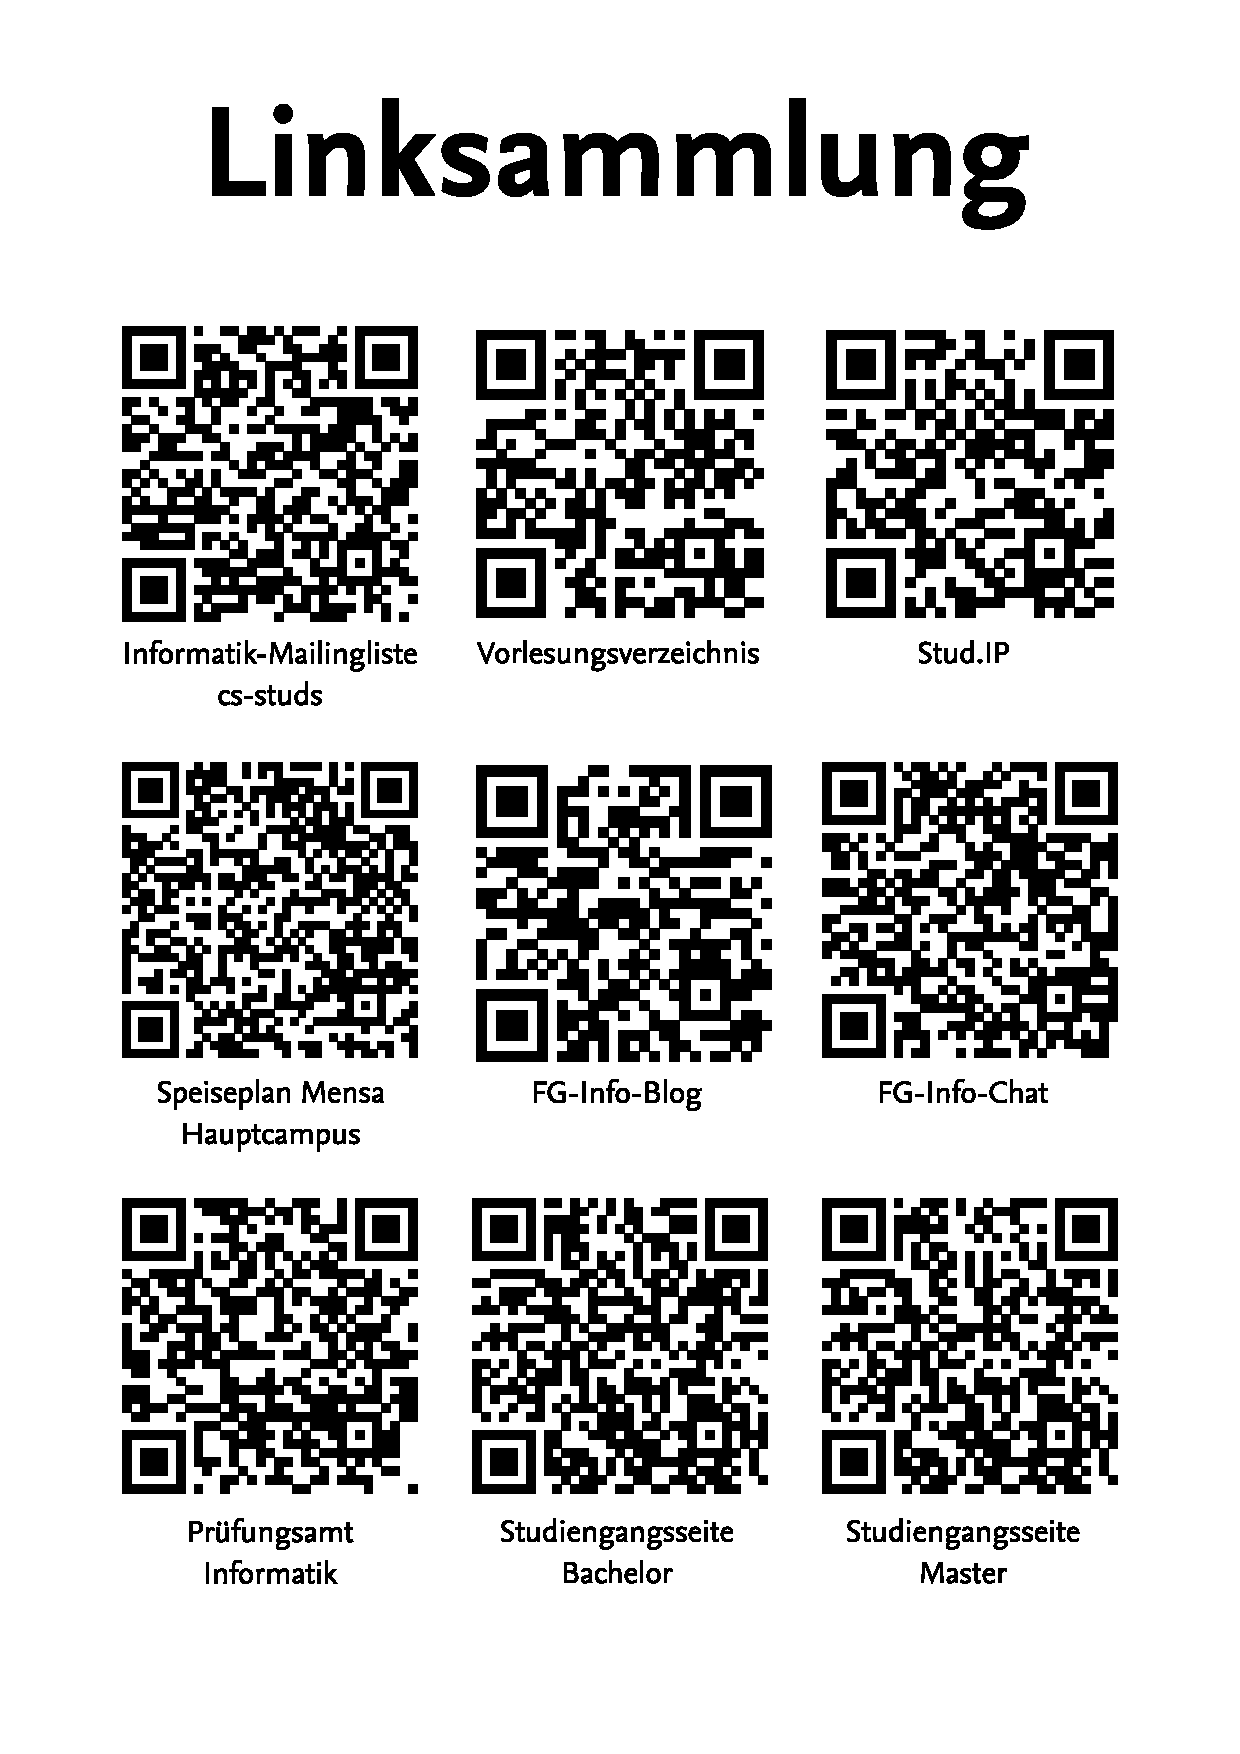
\includepdf[pages={1}]{bilder/Quicklinks/quicklinks.pdf}
		\newpage

		\begin{center}
			\includegraphics[width=\textwidth]{bilder/fg-logo/fg-logo.pdf}
		\end{center}

		\section*{Impressum}
		\label{impressum}
		% !TEX root = ../1-te.tex

\begin{description}
\item[Herausgeber:]
	Fachgruppe Informatik\\
	c/o AStA der TU Braunschweig\\
	Katharinenstraße 1\\
	38106 Braunschweig\\
	Tel.: 0531/391-4569\\
	E-Mail: \verHref{8}{mailto:fginfo@tu-bs.de}{fginfo@tu-bs.de}\\
	Webseite: \fginfoUrl
\item[Fachgruppenrat Informatik:] Nora~Widdecke, Thole~Goesmann, David~Hellmers, Nico~Grashoff, Eva~Vanessa~Bolle, Lucy~Wöbbekind \tocheck{8}{Aktuelle Mitglieder des FG-Rats einfügen}
\item[Cover:] Sophia Scholtka, Rebecca Finster, Eva Vanessa Bolle

\item[Comics:] Randall Munroe -- XKCD (\verUrl{8}{http://xkcd.com/})
\end{description}


		\vfill
		\xkcd{width=.9\textwidth}{devotion_to_duty}



	\clearpage
	\enlargethispage{5em}
	\input{texte/stundenplan/style_bunt}
	\section*{Einführungs- und Orientierungsveranstaltung zum Semesterbeginn}

\tocheck{8}{Stundenpläne überarbeiten}


\begin{savenotes}

\subsubsection*{6. April -- 10. April}

\begin{centering}
\begin{stundenplan}{18}{5.5}{9}{00}{17}{00} % width, height, starth, startmin, endh, endmin
	\Termin{Ersti-Frühstück\footnote[1]{Bitte eigenes Geschirr, Besteck und Tasse mitbringen}}
		{10:00, Plaza (IZ\footnote[2]{
			IZ:~Informatik-Zentrum,~Mühlenpfordstr.~23~|
			Mensa~1:~Katharinenstraße~1~| 
			%Eintracht-Stadium:~Hamburger~Str.~21~|
			PK:~Pockelstr.~| 
			SN:~Schleinitzstr.~| 
			Tentomax:~Konstantin-Uhde-Straße~| 
			%BI:~Campus~Nord,~Bienroder~Weg~97~| 
			Campusplan:~\verUrl{9}{https://campusplan.tu-braunschweig.de}
			\label{rooms}}~1.~OG)
		}{0}{10}{00}{11}{15}{fgTermin}
	\Termin{Stundenplanbauen}{11:00, IZ~160\footref{rooms}}{0}{11}{15}{13}{00}{fgTermin}
	\termin{Informatik-Vorkurs}{}{0}{13}{00}{17}{00}{uniTermin}

	\termin{Informatik-Vorkurs}{}{1}{9}{00}{13}{00}{uniTermin}
	\Termin{Mensa-Besuch}{13:00 -- 14:00, Mensa 1\footref{rooms}}{1}{13}{00}{14}{15}{fgTermin}
	\Termin{Campustour}{14:00, Treffen Foyer IZ\footref{rooms}}{1}{14}{15}{17}{00}{fgTermin}

	\termin{Informatik-Vorkurs}{}{2}{9}{00}{13}{00}{uniTermin}
	\Termin{Nachmittags-programm}{14:00, du kannst zwischen mehreren Optionen auswählen}{2}{14}{00}{17}{00}{fgTermin}
	\abendtermin{Linux-Install-Party}{17:00, IZ~160\footref{rooms}}{2}{fgTermin}

	\termin{Informatik-Vorkurs}{}{3}{9}{00}{13}{00}{uniTermin}
	\Termin{Nachmittags-programm}{14:00, du kannst zwischen mehreren Optionen auswählen}{3}{14}{00}{17}{00}{fgTermin}
	\abendtermin{Kneipentour}{19:00, Start Haupteingang der Mensa 1\footref{rooms}}{3}{fgTermin}

	%\termin{Informatik-Vorkurs}{}{4}{11}{00}{16}{00}{uniTermin} %Feiertag im Sommer2020	
\end{stundenplan}
\end{centering}

\vskip-100ex

\subsubsection*{13. April -- 17. April}

\begin{centering}
\begin{stundenplan}{18}{9}{8}{00}{16}{00} % width, height, starth, startmin, endh, endmin
	\termin{Analysis (V)}{PK~2.2\footref{rooms}}{0}{11}{30}{13}{00}{vlTermin}
	\Termin{Erstibegrüßung der Informatik}{13:15 -- 14:15, PK~2.2\footref{rooms}}{0}{13}{15}{14}{30}{uniTermin}

	\termin{Algebra (V)}{PK~2.2\footref{rooms}}{1}{9}{45}{11}{15}{vlTermin}
	\termin{Analysis (V)}{PK~2.2\footref{rooms}}{1}{11}{30}{13}{00}{vlTermin}

	\termin{Programmieren (V)}{Tentomax\footref{rooms}}{2}{8}{00}{9}{30}{vlTermin}
	\termin{Logik (V)}{PK 2.2\footref{rooms}, \emph{Letzter Termin für die Anmeldung zur Erstifahrt}}{2}{9}{45}{11}{15}{vlTermin}
	\termin{Programmieren (Ü)}{SN 19.1\footref{rooms}}{2}{11}{30}{13}{00}{vlTermin}
	\Termin{Infobörse für Erstsemester}{11:00 -- 16:00, Wiese vor der Mensa}{2}{13}{00}{16}{00}{uniTermin}

	\abendtermin{Spieleabend}{19:00, Flur vor IZ~150\footref{rooms}}{2}{fgTermin}

	\Termin{Treffen der Medizininformatiker}{
		15:00, IZ 404\footref{rooms}, \emph{
			Nur für Medizininformatikstudierende\footnote[3]{Um Anmeldung bei wird gebeten. Wenn du Medizininformatik studierest und teilnehmen willst, schicke eine Mail an ute.zeisberg@plri.de}
		}
	}{3}{14}{15}{16}{00}{uniTermin}


	\termin{Algebra (Ü)}{PK 2.2\footref{rooms}}{4}{8}{00}{9}{30}{vlTermin}
	\termin{Analysis (Ü)}{PK 2.2\footref{rooms}}{4}{9}{45}{11}{15}{vlTermin}
	\Termin{Abfahrt Erstifahrt}{Foyer IZ\footref{rooms}}{4}{13}{30}{14}{30}{fgTermin}

	\Termin{Erstifahrt}{Naturfreundehaus St. Andreasberg im Harz, Abreise Sonntag ab Mittag}{5}{0}{0}{24}{0}{fgTermin}

	% \Termin{Zentrale Erstibegrüßung}{9:00, Eintracht-Stadium}{0}{8}{45}{10}{00}{uniTermin}
	% \Termin{Infobörse}{10:30 -- 12:00, Altgebäude \& Audimax}{0}{10}{15}{11}{30}{uniTermin}
	% \termin{Lineare Algebra (V)}{PK~2.2\footref{rooms}}{0}{11}{30}{13}{00}{vlTermin}
	% \Termin{Erstibegrüßung der Informatik}{13:15 -- 14:15, PK~2.2\footref{rooms}}{0}{13}{15}{14}{30}{uniTermin}
	% \termin{Programmieren (V)}{PK~15.1\footref{rooms}}{0}{15}{00}{16}{30}{vlTermin}
	% \abendtermin{Uniweite Erstsemesterparty}{Diskothek Jolly Time}{0}{uniTermin}

	% \termin{Studium Generale}{Verteilt über Hauptcampus}{1}{10}{00}{16}{00}{uniTermin}
	% \abendtermin{Spieleabend}{19:00, Flur vor IZ~150\footref{rooms}, \emph{Letzter Termin für die Anmeldung zur Erstifahrt}}{1}{fgTermin}

	% \termin{Diskrete Mathematik (V)}{PK~2.2\footref{rooms}}{2}{9}{45}{11}{15}{vlTermin}
	% \termin{Lineare Algebra (V)}{PK~2.2\footref{rooms}}{2}{15}{00}{16}{30}{vlTermin}

	% \termin{Programmieren (Ü)}{PK~15.1\footref{rooms}}{3}{8}{00}{9}{30}{vlTermin}

	% \termin{Lineare Algebra (Ü)}{PK~2.2\footref{rooms}}{4}{9}{45}{11}{15}{vlTermin}
	% \Termin{Abfahrt Erstifahrt}{14:00, Foyer IZ\footref{rooms}}{4}{13}{30}{14}{30}{fgTermin}

	% \Termin{Erstifahrt}{Naturfreundehaus St. Andreasberg im Harz, Abreise Sonntag ab Mittag}{5}{0}{0}{24}{0}{fgTermin}
\end{stundenplan}

\end{centering}

%\enlargethispage{\baselineskip}
\end{savenotes}


\end{document}
